\documentclass[12pt,a4paper,table]{report}
\usepackage{fontspec}
\usepackage{fullpage}
\usepackage{hyperref}
\usepackage{array}
\usepackage{url}
\usepackage{latexsym}
\usepackage{amsmath}
\usepackage{pgf}
\usepackage{pgfplots}
\usepackage{pgfplotstable}
\usepackage{algorithm2e}
\usepackage{hhline}
\usepackage{multirow}
\usepackage{multicol}
\usepackage{subcaption}
\usepackage{cprotect}
\usepackage{color}
\usepackage{adjustbox}
\usepackage{tikz}
\usepackage{tikz-qtree}
\usepackage{tikz-dependency}
\usepackage{titling}
\usepackage{pdfpages}
\usepackage{rotating}
\usepackage{setspace}
\usepackage{collcell}
\usepackage{etoolbox}
\usepackage{booktabs}
\usepackage{float}
\usepackage[round]{natbib}
\usetikzlibrary{shapes,fit,calc,er,positioning,intersections,decorations.shapes,mindmap,trees}
\tikzset{decorate sep/.style 2 args={decorate,decoration={shape backgrounds,shape=circle,
      shape size=#1,shape sep=#2}}}
\pgfplotsset{select coords between index/.style 2 args={
    x filter/.code={
        \ifnum\coordindex<#1\def\pgfmathresult{}\fi
        \ifnum\coordindex>#2\def\pgfmathresult{}\fi
    }
}}

\newfontfamily\hebfont[Script=Hebrew, Scale=MatchUppercase]{FreeSans}
\newcommand{\heb}[1]{\bgroup\textdir TRT\hebfont #1\egroup}
\newcommand{\m}[1]{\mathbf{#1}}%

\newcommand{\parser}[1]{TUPA\textsubscript{#1}}
\newcommand{\secref}[1]{Section~\ref{#1}}
\newcommand{\figref}[1]{Figure~\ref{#1}}
\newcommand{\tabref}[1]{Table~\ref{#1}}
\DeclareMathOperator*{\argmin}{argmin}
\DeclareMathOperator*{\argmax}{argmax}
\SetKwRepeat{Do}{do}{while}

% for confusion matrix
\newcommand{\ApplyGradient}[1]{%
  \pgfmathsetmacro{\PercentColor}{(#1-0)/63.88}%
  \pgfmathsetmacro{\PercentInverse}{ifthenelse(\PercentColor > 70, 0, 100)}%
  %\textcolor{black!\PercentColor}{#1}
  \edef\x{\noexpand\cellcolor{red!\PercentColor}}\x\textcolor{black!\PercentInverse}{#1}%
}
\newcolumntype{R}{>{\collectcell\ApplyGradient}{c}<{\endcollectcell}}

\hyphenation{SemEval}
\hyphenation{PARSEVAL}
\hyphenation{DAGParser}
\hyphenation{TurboSemanticParser}
\hyphenation{MaltParser}
\hyphenation{UDPipe}
\hyphenation{CoNLL-U}

\renewcommand\cite{\citep}      % to get "(Author Year)" with natbib    
\newcommand\shortcite{\citeyearpar}% to get "(Year)" with natbib    
\newcommand\newcite{\citet}     % to get "Author (Year)" with natbib

\title{
\textbf{Universal Semantic Parsing with Neural Networks} \\
\vspace{2cm}
{\large Thesis submitted for the degree of \\
``Doctor of Philosophy''}
}
\author{
By \\
Daniel Hershcovich
\vspace{2cm}
}
\date{
Submitted to the Senate of the Hebrew University \\
February, 2019
}

\onehalfspacing

\begin{document}

\maketitle
\maketitle
\clearpage
\title{}
\author{
This work was carried out under the supervision of: \\
Prof. Ari Rappoport and Dr. Omri Abend
}
\date{}
\maketitle

\section*{Acknowledgments}

Even before I started my studies at the PhD program of
the Edmond and Lily Safra Center for Brain Sciences
(then the Interdisciplinary Center for Neural Computation),
I was interested in human language in general and learning languages
in particular, an interest I found early on that I shared with who became
my (first) PhD advisor, Ari Rappoport, to whom I am grateful for the
insightful conversations all along this process.
I am of course also indebted to my second advisor, Omri Abend,
whose shared interests with me and Ari have led to a fruitful
research project, which is still ongoing and I hope will continue for
many years.
They have set a very high standard, to which I continuously strive
and to which I surely owe much of my success so far.
I also thank my PhD committee members, Roi Reichart and Yoav Goldberg,
whose invaluable advice has shaped my research direction in the best way possible.

I sincerely appreciate the support of the ELSC staff and students,
and particularly the members of my year,
Adar Adamsky, Jonathan Bain, Haran Shani, Matan Holtzer, Henrike Horn, Adi Kol,
Ori Lavi Rotbain, Nimrod Levin, Oren Peles, Pnina Rappel, Benjamin Weiner, and
Noga Zaslavsky, whose company since the early stages of my graduate studies
has given me a sense of belonging and comfort.
I also thank the many other friends I made during my studies, including Nora Vrieler,
Ana Polterovich, Johannes Niediek, Dan Valsky, Nova Fandina and Stav Yardeni,
for their support.

My gratitude also goes to Roy Schwartz, who shared a great deal of his
experience with me and helped me become confident in my ideas, and to
Elior Sulem, who has accompanied me as a student in the lab and with whom
I shared a considerable part of my time there.
I would also like to thank past and current lab members, including Oren Tsur,
Eva Kimel, Dana Rubinstein, Saggy Herman, Effi Levi, Leshem Choshen, Zohar Aizenbud,
Aviram Stern, Adi Bitan and Michal Kessler, who have made these few years both
pleasant and interesting.
I must also express my gratitude towards Dotan Dvir and the UCCA annotation team,
without which this work would simply have not been possible.

Finally, I owe my deepest gratitude to my family for their support along the way,
and to my partner Michal for her endless love, patience and understanding,
which I value greatly.

\pagebreak

\section*{Abstract}

A major scientific effort is dedicated to \textit{natural language understanding},
which aims to be able to comprehend text, reason about it, and act upon it
in an intelligent way.
While specific use-cases or benchmarks can be solved with relatively simple
systems, which either ignore word order (``bag-of-words'' models) or treat
it as a simple linear structure
(such as the popular sequence-to-sequence framework allowing neural networks
to learn tasks in an end-to-end fashion),
understanding human language in general
requires a hierarchical representation of meaning.
Constructing this representation from text has been the goal of an extensive
line of work in \textit{semantic parsing}.
While many semantic representation schemes have been proposed,
they share many of their basic distinctions, such as between predicates
(relations, states and events) and arguments (participants).

This thesis focuses on a particular semantic representation scheme called
\textit{Universal Conceptual Cognitive Annotation} (UCCA),
whose main design principles are support for all major linguistic semantic phenomena,
cross-linguistic applicability, stability across translations,
ease of annotation (even by those who are not experts in linguistics),
and a modular architecture supporting multiple layers of semantic annotation.
A fully automatic parser is presented, and evaluated on multiple languages
(English, French and German).
The parser, titled ``TUPA'' (transition-based UCCA parser),
is able to learn very general graph structures:
directed acyclic graphs over token sequences with non-terminal nodes for complex
units, where these may cover discontinuous terminal yields.
This general class of graphs covers the structures annotated in UCCA,
as well as other representation schemes.
TUPA is implemented as a transition-based parser, whose transition system
supports these structural properties.
Its transition classifier is a neural network equipped with a
bidirectional long short-term memory (BiLSTM) module for calculating
feature representations for the input.
In an extensive comparison to conversion-based methods, as well as
other classifier implementations, TUPA is shown to outperform all baselines
in the task of UCCA parsing in both in-domain and out-of-domain settings
in three languages.

The parser is subsequently applied to two other semantic representation schemes,
DM and AMR, and to syntactic dependencies in the Universal Dependencies (UD)
scheme. This demonstrates that the flexible parser is usable not just for UCCA
parsing.
Furthermore, training TUPA in a multitask setting on all of these schemes
improves its UCCA parsing accuracy, by effectively learning generalizations
across the different representations:
a shared model is thus able to apply semantic distinctions in one task,
which have been learned for another.

Finally, in an empirical comparison of
the content of semantic and syntactic representations, we discover several
aspects of divergence, i.e., differences in the content captured by these schemes.
These have profound impact on the potential
contribution of syntax to semantic parsing, and on the usefulness of each of
the approaches for semantic tasks in natural language processing.

I see semantic parsing as a means for computers to learn language.
While different representations focus on different distinctions and do so
with formally different structures, they share an overall goal,
which is to support natural language processing applications,
such as classifying text into categories,
tagging it for linguistic properties,
performing inference and reasoning,
and generating new text according to some constraints
(e.g., machine translation).
The combined datasets annotated in every representation are an invaluable
resource, which, used effectively, can greatly boost our achievements in
language understanding and processing.

\pagebreak

\tableofcontents

\chapter{Introduction}

Natural language processing (NLP) or computational linguistics (CL)
is a sub-field of computer science with two main goals:
(1) developing methods for performing linguistic tasks automatically
so that solutions can be engineered for better human-computer interface
or analysis of large amounts of natural language data;
(2) computational modeling and study of natural language to answer linguistic questions.

Applications in NLP include classifying text into categories
(such as spam/non-spam, by topic, by author properties, or by
the sentiment expressed in it),
tagging it for linguistic properties (such as part-of-speech, i.e., noun/verb/etc.),
building abstract representations for it (for linguistic research or for
more readily integrating them into downstream applications)
and generating new text according to some constraints (for example,
machine translation is the task of generating
text in a target language given source language text;
text simplification is the task of generating simple text with approximately the same
meaning as given complex text).

Semantic tasks in natural language processing, such as machine translation and
sentiment analysis, require understanding the meaning of text. Since text is
merely a sequence of words, it has to be represented in a way that will convey
its meaning. One simple approach, known as the bag-of-words model, looks only
at which words occur in the text.
This can already provide
substantial information about the meaning, but it ignores the order of words,
which clearly conveys important information as well. The n-gram model counts
sequences of words with regard to their order, incorporating at least some of
the meaning encoded in the text structure.
Many models treat text as a simple linear structure,
such as the popular sequence-to-sequence framework allowing neural networks
to learn tasks in an end-to-end fashion.

Specific use-cases or benchmarks can be solved with such relatively simple
systems, which either ignore word order or make simplifying assumptions about structure.
However, understanding human language in general
requires a hierarchical representation of meaning,
as an undeniable part in the
meaning of language resides in its hierarchical structure.

Indeed, a major effort in NLP is dedicated to \textit{natural language understanding},
which aims to be able to comprehend text, reason about it, and act upon it
in an intelligent way.
For example, executable semantic parsing\footnote{Two conceptually distinct
tasks are termed \textit{semantic parsing}: parsing into
executable representations, such as SQL; and parsing into descriptive meaning
representation, such as AMR or UCCA.
We disambiguate by referring to the former as \textit{executable semantic parsing}.}
is the task of generating logical meaning representations in the form of code, such as
SQL or Python, which can then be executed against a knowledge base to perform
tasks or answer questions.
In general, constructing a hierarchical representation from text has been the
goal of an extensive line of work in \textit{semantic parsing}.
While many semantic representation schemes have been proposed,
they share many of their basic distinctions \citep{abend2017state},
such as between predicates
(relations, states and events) and arguments (participants).

Syntax is a way to
model this structure formally. Using syntactic features can improve the
performance in semantic tasks.
However, syntactic annotations suffer from limitations, since they do not
represent the semantic structure of text directly. Simple manipulations such as
switching from an active construction to a passive one, which nearly do not
alter the meaning of text, can yield a significantly different syntactic
structure. Moreover, the same syntactic construct can express conceptually
distinct semantic structures: while ``chairmen of parliaments'' and
``dozens of parliaments'' have the same syntactic structure, semantically
they are quite distinct.

Universal Dependencies \citep{nivre2016universal}
is a \textit{syntactic} dependency scheme aiming for cross-lingual consistency,
whose annotation is often similar to the common practice in semantic treebanks
(Figure~\ref{fig:original_example_ud}).
See Table~\ref{tab:ud} for a concise description of UD relations.

\begin{figure}[t]
  \centering
    \begin{dependency}[text only label, label style={above,font=\tt}, font=\small]
    \begin{deptext}[column sep=.8em]
    Glad \& I    \& called \& before \& I    \& arrived \& with \& my   \& box  \& to   \& ship \& . \\
    \end{deptext}
\deproot{1}{root}
\depedge{3}{2}{nsubj}
\depedge{1}{3}{ccomp}
\depedge{6}{4}{mark}
\depedge{6}{5}{nsubj}
\depedge{3}{6}{advcl}
\depedge{9}{7}{case}
\depedge{9}{8}{nmod:poss}
\depedge{6}{9}{obl}
\depedge{11}{10}{mark}
\depedge{9}{11}{acl}
\depedge[edge unit distance=1.5ex]{1}{12}{punct}
    \end{dependency}
\caption{Example UD tree (\texttt{reviews-372665-0003} from UD\_English-EWT), demonstrating practices common in semantic annotation:
linking content words to content words, and preference of lexical heads over functional ones.
\label{fig:original_example_ud}}
\end{figure}

\section{Semantic Representations}\label{sec:intro_semantic_reps}

As opposed to syntactic annotation, which reflects language-specific formal
patterns, semantic annotation corresponds to a higher level of cognitive
processing, and the same framework can potentially apply to any language.
Moreover, a rich semantic annotation scheme may be better than
syntactic annotation as an input for applications that attempt to solve a
semantic task, due to their tighter relation to the meaning of the text.
Ideally, a semantic representation abstracts away from detail that does not affect meaning:

\begin{center}
    \fbox{\textrm{rest}} $\approx$ \fbox{\textrm{take a break}}
    
    \fbox{\textrm{graduation}} $\approx$ \fbox{\heb{סיים את הלימודים}}
\end{center}

While syntactic description does not suffice to discern meaning from natural language,
some syntactic formalisms provide a theory of the \textit{syntax-semantics interface}.
Examples include analyses using Head-driven Phrase Structure Grammar \cite[HPSG;][]{PandS:94},
Combinatory Categorial Grammar \cite[CCG;][]{Steedman:00} and Tree-Adjoining Grammars
\cite[TAG;][]{Joshi:97}.
They have been used as a basis for meaning representation
by defining compositional semantics on top of them:
\citet{Flic:00} introduced the LinGO English Resource Grammer (ERG),
a broad-coverage, linguistically precise HPSG-based grammar of English,
which is semantically grounded in Minimal Recursion Semantics \cite[MRS;][]{copestake2005minimal},
a form of flat semantic representation capable of supporting underspecification.

\citet{bos2005towards,bos2008wide,bos2015open} introduced the Boxer parser,
which uses syntactic analysis in the form of CCG derivations
to compositionally derive Discourse Representation Structures.
Discourse Representation Theory \cite[DRT;][]{kamp2013discourse}
is a general framework for representing the meaning of sentences and discourse,
which can handle multiple linguistic phenomena including anaphora, presuppositions, and temporal expressions. The basic meaning-carrying
units in DRT are Discourse Representation Structures (DRSs), which are recursive formal meaning structures that have a model-theoretic interpretation and can be translated into first-order logic. Basic DRSs consist
of discourse referents representing entities in the discourse, and discourse conditions
representing information about discourse referents.

In semantic role labeling \cite{Baker:98,Palmer:05},
predicates and their arguments are annotated and classified into specific roles.
While earlier work on semantic parsing has mostly concentrated on shallow semantic analysis,
focusing on semantic role labeling of verbal argument structures,
the focus has shifted to parsing of more elaborate representations that account
for a wider range of phenomena. 
Most closely related to my work are Broad-Coverage Semantic Dependency Parsing (SDP)
frameworks, such DM (DELPH-IN MRS), converted from
DeepBank \cite{flickinger2012deepbank}, a corpus of hand-corrected parses from LinGO ERG.
It addresses a wide range of semantic phenomena,
and supports discontinuous units and multiple parents \citep{oepen2016towards}.
However, SDP uses bi-lexical dependencies
(meaning every relation or edge is between a pair of words),
disallowing non-terminal nodes (see below),
and thus faces difficulties in supporting
structures that have no clear head, such as coordination \citep{Ivanova2012who}.
Figure~\ref{fig:syntactic_semantic_dependencies} example shows {syntactic}/{semantic} bi-lexical dependencies for the sentence ``While driving, I listen to podcasts''.

    \begin{figure}\centering
    \begin{dependency}
        \begin{deptext}[column sep=1.5em,ampersand replacement=\^,font=\rmfamily]
          While \^ driving \^ , \^ I \^ listen \^ to \^ podcasts \\
        \end{deptext}
        \depedge[edge below,edge unit distance=3ex]{1}{2}{ARG2}
        \depedge[edge below,edge unit distance=3ex]{5}{4}{ARG1}
        \depedge[edge below,edge unit distance=2ex, edge end x offset=-2pt]{1}{5}{ARG1}
        \deproot[edge below,edge unit distance=3ex]{5}{top}
        \depedge[edge below,edge unit distance=4ex, edge start x offset=-1pt, edge end x offset=3pt]{5}{7}{ARG2}
        \depedge[edge below,edge unit distance=3ex, edge end x offset=5pt]{6}{5}{ARG1}
        \depedge[edge below,edge unit distance=3ex]{6}{7}{ARG2}
        \depedge[edge unit distance=3ex]{2}{1}{case}
        \depedge[edge unit distance=3ex]{2}{3}{punct}
        \depedge[edge unit distance=3ex]{5}{4}{nsubj}
        \depedge[edge unit distance=3ex, edge end x offset=-2pt]{5}{2}{obl}
        \depedge[edge unit distance=3ex]{7}{6}{case}
        \deproot[edge unit distance=4ex]{5}{root}
        \depedge[edge unit distance=4ex]{5}{7}{obl}
    \end{dependency}
    \caption{Top: syntactic dependencies in the Universal Dependencies framework.
    Bottom: semantic dependencies in the DM (DELPH-IN MRS) framework.}\label{fig:syntactic_semantic_dependencies}
    \end{figure}

Another line of work addresses parsing into Abstract Meaning Representations
\citep[AMRs;][]{banarescu2013abstract,flanigan2014discriminative,vanderwende2015amr,pust2015parsing,artzi2015broad,wang2015transition,wang-EtAl:2016:SemEval,wang-xue-pradhan:2015:ACL-IJCNLP,zhou2016amr,damonte-17,N18-1104}.
AMR represents a rich set of semantic distinctions in a single homogeneous formalism,
including named entity recognition and linking, semantic role labeling, and (indirectly)
coreference resolution.
While sharing much of my work's motivation,
AMR does not ground its units in the words and constituents of the text.
This complicates the parsing task, as it requires
that the alignment between words and logical symbols be automatically
(and imprecisely) detected.
Furthermore, it complicates applications using the meaning representation,
as it is not immediately clear what portion of the text corresponds to what portion
of the meaning representation, which may be necessary for tasks such as
rephrasing, translation or evaluation of parts of the text.

While many of the parsing approaches mentioned above rely on a theory of syntax-semantics
interface, on syntactic features or on syntactic pre-processing for semantic parsing,
some semantic annotation schemes and parsing approaches attempt to represent the meaning of 
natural language utterances directly.
While the parser presented in this thesis does make use of syntactic features,
it largely belongs to this category, as it makes no or minimal assumptions about the
relation between the syntactic and the semantic structures.
This ``purist'' approach is attractive, as it avoids biases and language-specific
properties that might be introduced by using a specific syntactic framework.

\section{Universal Conceptual Cognitive Annotation}\label{sec:intro_ucca}

Universal Cognitive Conceptual Annotation \citep[UCCA;][]{abend2013universal}
is a cross-linguistically applicable semantic representation scheme.
It covers the predicate-argument
structures evoked by predicates of all grammatical categories, the inter-relations between them,
as well as other major linguistic phenomena.
UCCA has demonstrated applicability to multiple languages,
rapid annotation \citep{abend2017uccaapp},
and benefit for various applications:
evaluation of machine translation \citep{birch2016hume},
evaluation of grammatical error correction \citep{choshen2018reference},
as demonstrated in Figure~\ref{fig:usim},
evaluation of structural text simplification \citep{sulem2018semantic}
and text simplification \citep{sulem2018simple}.

\begin{figure}\centering
            \begin{tikzpicture}[level distance=7mm, sibling distance=6mm,
                every node/.append style={font=\rmfamily},
            	every circle node/.append style={fill=black}]
                \begin{scope}[frontier/.style={distance from root=23mm},
                    edge from parent path={(\tikzparentnode.center)
                	.. controls +(0,-.25) and +(0,.25) .. (\tikzchildnode.north)},
                    edge from parent/.append style={nodes={font=\scriptsize}}]
                \Tree [.\node [circle] (root u) {};
                  \edge node [auto=right]{L}; \node (After u) {After};
                  \edge node[auto=left]{H};
                  [.\node [circle,xshift=8mm](graduation John u) {};
                    \edge node[auto=right]{P}; \node (graduation u) {graduation};
                  ]
                  \edge node[auto=left]{H};
                  [.\node [circle](John moved to Copenhagen u) {};
                    \edge node[auto=right]{A}; \node (John u) {John};
                    \edge node[auto=left]{P}; \node (moved u) {moved};
                    \edge node[auto=left]{A};
                    [.\node [circle](to Copenhagen u) {};
                      \edge node[auto=right]{R}; \node (to u) {to};
                      \edge node[auto=left]{C}; \node (Copenhagen u) {Copenhagen};
                    ]
                  ]
                ]
                \draw[dashed] (graduation John u) to node[auto] {\scriptsize A} (John u);
                \end{scope}
                  \begin{scope}[xshift=2cm,yshift=-58mm,grow'=up,level distance=9mm,
                      sibling distance=4mm, frontier/.style={distance from root=19mm},
                      edge from parent path={(\tikzparentnode.center) ..
                      controls +(0,.25) and +(0,-.25) .. (\tikzchildnode.south)},
                      edge from parent/.append style={nodes={font=\scriptsize}}]
                  \Tree [.\node [circle] (rootd) {};
                    \edge node[auto=left]{H};
                    [.\node [circle,xshift=-5mm] (John siyem et halimudim d) {};
                      \edge node[auto=left]{P}; \node (halimudim d) {\heb{הלימודים}};
                      \edge node[auto=left]{F}; \node (et d) {\heb{את}};
                      \edge node[auto=right]{D}; \node (siyem d) {\heb{שסיים}};
                    ]
                    \edge node [auto=left,anchor=south east]{L}; \node (ahrei d) {\heb{אחרי}};
                    \edge node[auto=right]{H};
                    [.\node [circle] (hu avar lecopenhagen d) {};
                      \edge node[auto=left,anchor=south east]{A}; \node (lecopenhagen d) {\heb{לקופנהגן}};
                      \edge node[auto=left]{P}; \node (avar d) {\heb{עבר}};
                      \edge node[auto=right]{A}; \node (John d) {\heb{ג'ון}};
                    ]
                  ]
                  \draw[dashed] (John siyem et halimudim d) to[out=-15,in=-150] node[above] {\scriptsize A} (John d);
                  \end{scope}
                  \begin{scope}[dashed,thick]
                    \draw (After u) to[out=-45,in=135] (ahrei d);
                    \draw (graduation u) to[out=-90,in=100] (John siyem et halimudim d);
                    \draw (John u) -- (John d);
                    \draw (moved u) to[out=-30,in=90] (avar d);
                    \draw (to Copenhagen u) to[out=-90,in=70] (lecopenhagen d);
                  \end{scope}
            \end{tikzpicture}
            \caption{Illustration for the cross-linguistic applicability of UCCA.}
\end{figure}
\begin{figure}\centering
                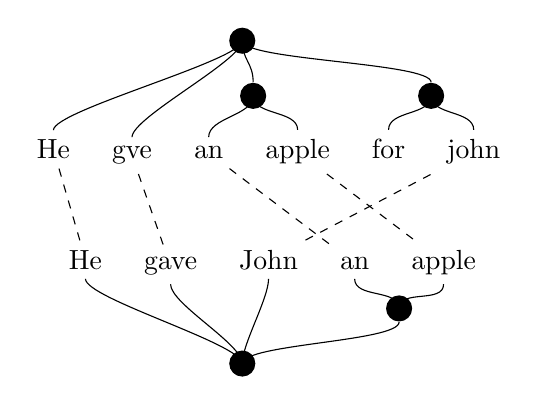
\begin{tikzpicture}[sibling distance=3mm, level distance=7mm,
                every node/.append style={font=\rmfamily},
            	every circle node/.append style={fill=black}]
                \begin{scope}[frontier/.style={distance from root=15mm},
            	edge from parent path={(\tikzparentnode.center) ..
                    controls +(0,-.25) and +(0,.25) .. (\tikzchildnode.north)}]
                \Tree [.\node [circle] (rootu) {};
                \edge node [auto=right]{}; \node (Heu) {He};
                \edge node[auto=right down]{}; \node (gve) {gve};
                \edge node[auto=right]{};
                [.\node [circle](an appleu) {};
                \edge node[auto=right]{}; \node (anu) {an};
                \edge node[auto=left]{}; \node (appleu) {apple};
                ]
                \edge node[auto=left]{};
                [.\node [circle](for john) {};
                \edge node[auto=right]{};\node (for) {for};
                \edge node[auto=left]{}; \node (john) {john};
                ]]
                \end{scope}
                \begin{scope}[yshift=-41mm,grow'=up,
                  frontier/.style={distance from root=12mm},
                  edge from parent path={(\tikzparentnode.center) ..
                  controls +(0,.25) and +(0,-.25) .. (\tikzchildnode.south)}]
                \Tree [.\node [circle] (rootd) {};
                \edge node [auto=left]{}; \node (Hed) {He};
                \edge node[auto=right]{}; \node (gave) {gave};
                \edge node[auto=right]{};\node (John) {John};
                \edge node[auto=right]{};
                [.\node [circle] (an appled) {};
                \edge node[auto=left]{}; \node (and) {an};
                \edge node[auto=right]{}; \node (appled) {apple};
                ]
                ]
                \end{scope}
                \begin{scope}[dashed]
                \draw (Heu) -- (Hed);
                \draw (gve) -- (gave);
                \draw (John) -- (john);
                \draw (anu) -- (and);
                \draw (appleu) -- (appled);
                \end{scope}
                \end{tikzpicture}
                \caption{UCCA for grammatical error correction evaluation.}\label{fig:usim}
\end{figure}

UCCA is a typologically-motivated scheme for analyzing abstract semantic structures in text. It aims to abstract away from grammatical particularities of a passage 
such that paraphrases, and translations tend to have similar UCCA structures.
Accordingly, UCCA has been studied with respect to meaning preservation in translation \citep{sulem2015conceptual},
and found to be more stable than phrase-structure syntactic annotation.
UCCA corpora are available for English, French and German, and pilot studies were conducted on a few languages more.\footnote{\scriptsize\url{https://github.com/UniversalConceptualCognitiveAnnotation}}
In English, data was annotated from Wikipedia, the book \textit{Twenty Thousand Leagues under the Sea}, and the English Web Treebank Web Reviews corpus (see Table~\ref{tab:data_english}).

\begin{table}
\centering
\begin{tabular}{l|r|rrr|r}
    & \multicolumn{1}{c|}{Wiki} & \multicolumn{3}{c|}{20K} & \multicolumn{1}{c}{EWT} \\
    & \multicolumn{1}{c|}{en} & \multicolumn{1}{c}{en} & \multicolumn{1}{c}{fr} & \multicolumn{1}{c|}{de} & \multicolumn{1}{c}{en} \\
    \hline
    \# sentences&5,141&492&492&6,514&3,520 \\
    \# tokens&158,739&12,638&13,021&144,529&51,042 \\
    \hline
    \# { non-terminal nodes}&62,002&4,699&5,110&51,934&18,156 \\
    \% {discontinuous}&1.71&3.19&4.64&8.87&3.87 \\
    \% {reentrant}&1.84&0.89&0.65&0.31&0.83 \\
    \hline
    \# edges&208,937&16,803&17,520&187,533&60,739 \\
    \% primary&97.40&96.79&97.02&97.32&97.32 \\
    \% remote&2.60&3.21&2.98&2.68&2.68
\end{tabular}
\caption{UCCA data statistics.}\label{tab:data_english}
\end{table}

\begin{figure}[ht]\small\centering
  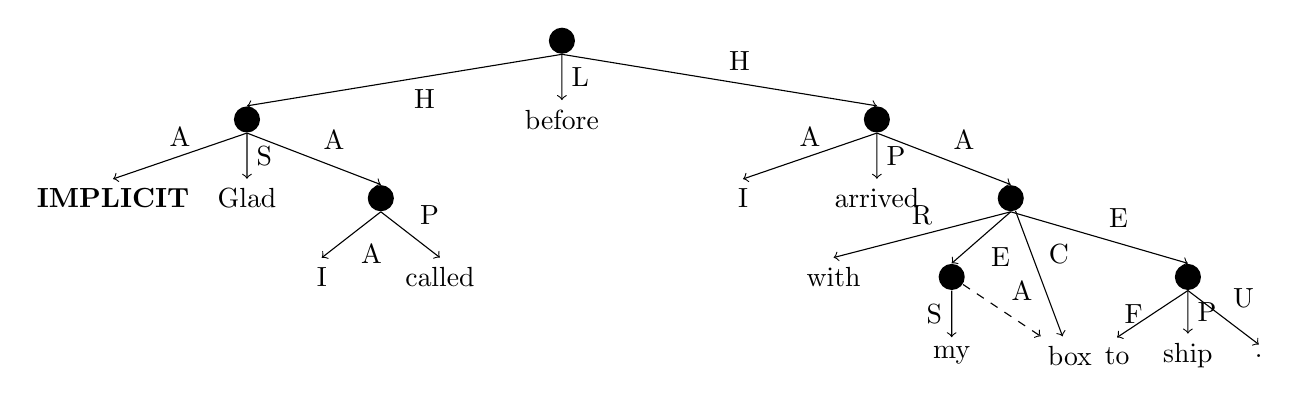
\begin{tikzpicture}[->,level distance=1cm,
  level 1/.style={sibling distance=4cm},
  level 2/.style={sibling distance=17mm},
  level 3/.style={sibling distance=15mm},
  level 4/.style={sibling distance=9mm},
  every circle node/.append style={fill=black}]
  \tikzstyle{word} = [font=\rmfamily,color=black]
  \node (1_1) [circle] {}
  {
  child {node (1_2) [circle] {}
    {
    child {node (1_16) [word] {\textbf{IMPLICIT}}  edge from parent node[above]  {A}}
    child {node (1_17) [word] {Glad}  edge from parent node[auto]  {S}}
    child {node (1_18) [circle] {}
      {
      child {node (1_19) [word] {I}  edge from parent node[auto]  {A}}
      child {node (1_20) [word] {called}  edge from parent node[auto]  {P}}
      } edge from parent node[auto]  {A}}
    } edge from parent node[auto]  {H}}
  child {node (1_3) [word] {before}  edge from parent node[auto]  {L}}
  child {node (1_4) [circle] {}
    {
    child {node (1_6) [word] {I}  edge from parent node[above]  {A}}
    child {node (1_7) [word] {arrived}  edge from parent node[auto]  {P}}
    child {node (1_8) [circle] {}
      {
      child {node (1_9) [word] {with}  edge from parent node[above]  {R}}
      child {node (1_10) [circle] {}
        {
        child {node (1_15) [word] {my}  edge from parent node[left]  {S}}
        } edge from parent node[auto]  {E}}
      child {node {}
        {
        child {node (1_11) [word] {box}  edge from parent [draw=none] {}}
        } edge from parent [draw=none] {}}
      child {node (1_12) [circle] {}
        {
        child {node (1_13) [word] {to}  edge from parent node[left]  {F}}
        child {node (1_14) [word] {ship}  edge from parent node[auto]  {P}}
        child {node (1_21) [word] {.}  edge from parent node[auto]  {U}}
        } edge from parent node[auto]  {E}}
      } edge from parent node[auto]  {A}}
    } edge from parent node[auto]  {H}}
  };
  \draw[dashed,->] (1_10) to node [auto] {A} (1_11);
  \draw[->] (1_8) to node [auto] {C} (1_11);
\end{tikzpicture}
\caption{UCCA example including an implicit node, where the subject of ``Glad'' is omitted.}\label{fig:implicit}
\end{figure}

   Formally, UCCA structures are directed acyclic graphs (DAGs) whose nodes (or {\it units}) correspond to (are \textit{anchored} by) words,
   or elements viewed as a single entity according to some semantic or cognitive consideration.
   Edges are labeled with \textit{categories}, indicating the role of a child in the relation the parent represents.
   See Table~\ref{tab:ucca} for a concise description of UCCA categories.
   A {\it Scene} is UCCA's notion of an event or a frame, and is a description of a movement, an action or a state which persists in time. 
   Every Scene contains one primary relation, which can be either a Process or a State. 
   Scenes may contain any number of Participants, a category which also includes abstract participants and locations.
   They may also contain temporal relations (Time), and secondary relations (Adverbials), 
   which cover semantic distinctions such as manner, modality and aspect.
   UCCA also supports \textbf{implicit units} which do not correspond to any tokens,
such as the implicit semantic subject of ``Glad'' in Figure~\ref{fig:implicit}.
The principal kind of unit is a \textbf{scene} denoting a situation mentioned in the sentence, typically involving a scene-evoking \textbf{predicate}, participants, and (perhaps) modifiers. 

   Scenes may be \textit{linked} to one another in several ways.
   First, a Scene can provide information about some entity,
   in which case it is marked as an Elaborator.
   This often occurs in the case of participles or relative clauses.
   For example, ``(child) who went to school'' is an Elaborator Scene
   in ``The child who went to school is John''.
   A Scene may also be a Participant in another Scene. For example, ``John went to school'' in the sentence: ``He said John went to school''. 
   In other cases, Scenes are annotated as Parallel Scenes (H), which are flat structures and may include a Linker (L), 
   as in: ``When$_L$ [he arrives]$_H$, [he will call them]$_H$''.

   Non-Scene units are headed by units of the category Center,
   denoting the type of entity or thing described by the whole unit.
   Elements in non-Scene units include Quantifiers (such as ``{\it dozens} of people'') and
   Connectors (mostly coordinating conjunctions).
   Other modifiers to the Center are marked as Elaborators.

Figure~\ref{fig:implicit} contains five scenes: one anchored by the State \textit{Glad}; one anchored by the Process \textit{called}; one anchored by the Process \textit{arrived}; one anchored by the Process \textit{ship}; and one anchored by the possessive pronoun \textit{my}, which indicates a stative possession relation.
A Participant (A) of a scene is typically an entity or location involved. 
Adverbials (D) modify scenes with respect to properties like negation, modality, causativity, direction, manner, etc., which do not constitute an independent situation or entity.
Temporal modifiers are labeled Time (T).

A scene can serve as a Participant within a larger scene: Figure~\ref{fig:implicit} embeds the ``called'' scene within the ``Glad'' scene.
A scene can also serve as an Elaborator of a non-scene unit:
``my'' and ``to ship'' in Figure~\ref{fig:implicit} are both Elaborators of ``box''.
Other relations between scenes are called \textbf{parallel linkage}: a unit consists of Parallel Scenes (H) and possibly Linkers (L) describing how they are related. This is seen at the top level of Figure~\ref{fig:implicit}, where the ``Glad'' and ``arrived'' scenes are parallel and the word ``before'' is a linker.

Other categories only apply under \textbf{non-scene units}, i.e., units with no predicate: a semantic head---the Center (C); modifiers of Quantity (Q); and other modifiers, called Elaborators (E).
A Connector (N) groups together multiple non-scene units into a larger unit, e.g., ``You and I'' in Figure~\ref{fig:changetheworld}.

\begin{figure}[ht]\small
  \begin{subfigure}{.45\textwidth}
  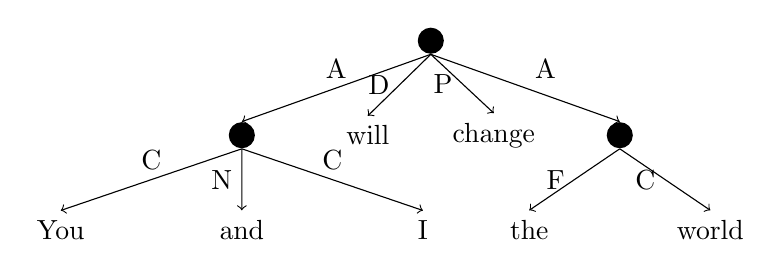
\begin{tikzpicture}[level distance=12mm, ->,
  level 1/.style={sibling distance=16mm},
  level 2/.style={sibling distance=23mm},
  level 3/.style={sibling distance=15mm},
      every node/.append style={midway}]
    \node (ROOT) [fill=black, circle] {}
      child {node [fill=black, circle] {}
      {
        child {node {You} edge from parent node[above] {C}}
        child {node {and} edge from parent node[left] {N}}
        child {node {I} edge from parent node[above] {C}}
      } edge from parent node[above] {A} }
      child {node {will} edge from parent node[left] {D}}
      child {node {change} edge from parent node[left] {P}}
      child {node [fill=black, circle] {}
      {
        child {node {the} edge from parent node[left] {F}}
        child {node {world} edge from parent node[left] {C}}
      } edge from parent node[auto] {A} }
      ;
  \end{tikzpicture}
  \caption{}\label{fig:changetheworld}
  \end{subfigure}\hfill
  \begin{subfigure}{.45\textwidth}
  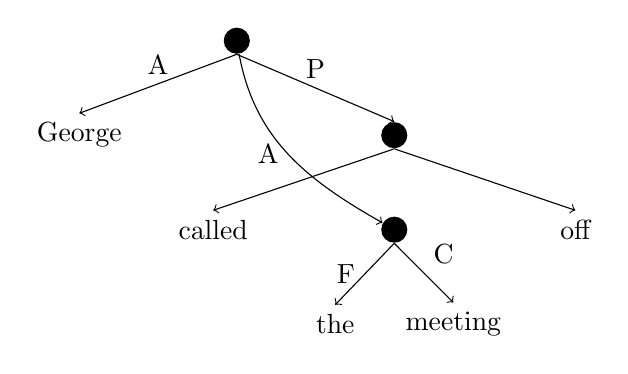
\begin{tikzpicture}[level distance=12mm, ->,
  level 1/.style={sibling distance=4cm},
  level 2/.style={sibling distance=23mm},
  level 3/.style={sibling distance=15mm},
      every node/.append style={midway}]
    \node (ROOT) [fill=black, circle] {}
      child {node {George} edge from parent node[above] {A}}
      child {node [fill=black, circle] {}
      {
      	child {node {called} edge from parent node[right] {}}
      	child {node (themeeting) [fill=black, circle] {}
        {
      	  child {node {the} edge from parent [black] node[left] {F}}
      	  child {node {meeting} edge from parent [black] node[auto] {C}}
      	} edge from parent[white]}
      	child {node {off} edge from parent node[above] {}}
      } edge from parent node[above] {P} }
      ;
    \draw[bend right,->] (ROOT) to[out=-30, in=200] node [left] {A} (themeeting);
  \end{tikzpicture}
  \caption{}\label{fig:calledoff}
  \end{subfigure}
  \caption{\label{fig:examples}
    UCCA examples.
    (\subref{fig:changetheworld}) includes a coordination construction (``You and I'').
    (\subref{fig:calledoff}) includes a discontinuous unit (``called ... off'').
  }
\end{figure}

Apart from the main semantic content of scenes, participants, and connectives, UCCA provides the categories: Relator (R) for grammatical markers expressing how a unit relates to its parent unit---in English, these are mainly prepositions and the possessive \textit{'s}; Function (F) for other grammatical markers with minimal semantic content, such as tense auxiliaries, light verbs, and articles; and Ground (G) for expressions expressing speaker perspective outside the propositional structure of the sentence.
The least contentful elements---Fs, and to a lesser extent Rs---are subject to considerable variation when paraphrasing or translating a sentence.
Punctuation tokens are attached to units as U, but are generally also regarded as non-content-bearing.

Note that in Figure~\ref{fig:calledoff}, the tokens of the unit \textit{called off} do not receive individual labels: this is called an \textbf{unanalyzable unit}, and is used for semantically opaque multi-word expressions.

\begin{figure}[ht]\small\centering
  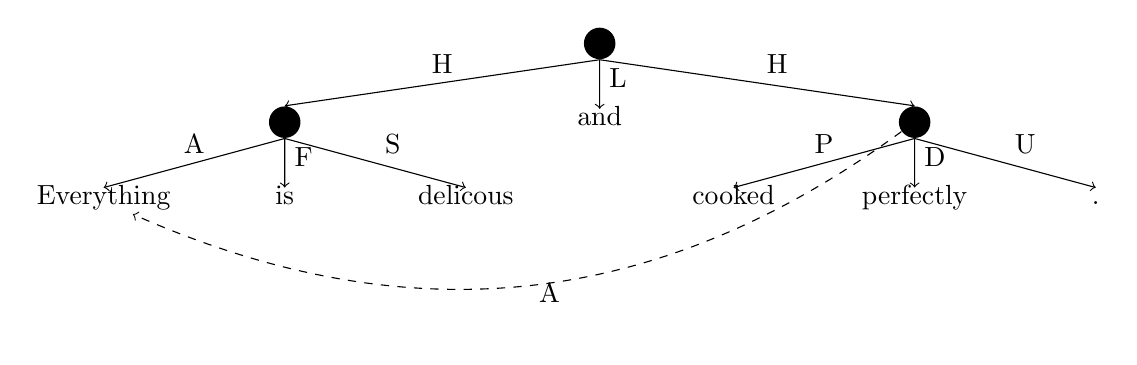
\begin{tikzpicture}[->,level distance=1cm,
  level 1/.style={sibling distance=4cm},
  level 2/.style={sibling distance=23mm},
  level 3/.style={sibling distance=15mm},
  every circle node/.append style={fill=black},
  every node/.append style={text height=.6ex,text depth=0}]
  \tikzstyle{word} = [font=\rmfamily,color=black]
  \node (1_1) [circle] {}
  {
  child {node (1_2) [circle] {}
    {
    child {node (1_8) [word] {Everything}  edge from parent node[above]  {A}}
    child {node (1_9) [word] {is}  edge from parent node[auto]  {F}}
    child {node (1_10) [word] {delicous}  edge from parent node[auto]  {S}}
    } edge from parent node[above]  {H}}
  child {node (1_3) [word] {and}  edge from parent node[auto]  {L}}
  child {node (1_4) [circle] {}
    {
    child {node (1_6) [word] {cooked}  edge from parent node[above]  {P}}
    child {node (1_7) [word] {perfectly}  edge from parent node[auto]  {D}}
    child {node (1_11) [word] {.}  edge from parent node[auto]  {U}}
    } edge from parent node[auto]  {H}}
  };
  \draw[dashed,->,bend left] (1_4) to node [auto] {A} (1_8);
\end{tikzpicture}
\caption{
    UCCA example including a remote edge (dashed),
    resulting in ``Everything'' having two parents.}\label{fig:remote}
\end{figure}

The solid edges in the UCCA graphs are called \textbf{primary edges}: the primary edges in UCCA always form a tree. 
\textbf{Remote edges}, such as the dotted edge from the possession scene unit to ``box'' in Figure~\ref{fig:implicit}
and the dotted A edge to ``Everything'' in Figure~\ref{fig:remote}, allow for additional relations, forming a DAG:
multiple parents are enabled exclusively by remote edges.
Remote edges are commonly used with attributive possessives and adjectives, and relative clauses, where the head of the noun phrase doubles as a semantic participant of the modifier scene. 
They also figure in multi-scene control constructions (\textit{John told Mary to leave}: \textit{Mary} is a primary participant of the telling scene and a remote participant of the leaving scene).

\section{UCCA Parsing}\label{sec:intro_ucca_parsing}

In order to represent the full range of semantic structures exhibited by
natural language, three properties should be supported: reentrancy,
representing arguments shared between predicates;
non-terminal nodes for multi-word units;
and discontinuity of semantic units in the text.

The first property, \textbf{reentrancy} (or \textbf{multiple parents}), is required for
representing arguments and relations (semantic units) that are shared between predicates.
For instance, in the sentence
``Everything is delicious and cooked perfectly'' (Figure~\ref{fig:remote}),
``Everything'' is an argument of both ``delicious''
and ``cooked perfectly'', yielding a DAG structure rather than a tree.

The second is \textbf{non-terminal nodes} for representing units
comprising more than one word (Figure~\ref{fig:changetheworld}).
While bi-lexical dependencies partially circumvent this requirement, by
representing complex units in terms of their headwords, they fall short
when representing units that have no clear head.
Frequent examples of such constructions include
coordination structures (e.g., ``\textit{You and I} will change the world''),
some multi-word expressions (e.g., ``The Haves and the \textit{Have Nots}''),
and prepositional phrases.
In these cases, dependency schemes often apply some annotation convention that
selects one of the sub-units
as the head, but as different head selections are needed for different purposes,
standardization problems arise \citep{Ivanova2012who}.
For example, selecting the preposition to head prepositional phrases yields better
parsing results \citep{Schwartz:12}, while the head noun can be more useful for
information extraction purposes.

Third, semantic units may be \textbf{discontinuous} in the text. For instance, in
``George \textit{called} the meeting \textit{off}'' (Figure~\ref{fig:calledoff}),
the phrasal verb ``called ... off'' forms a single semantic unit.
Discontinuities are also pervasive with other multi-word
expressions \citep{schneider2014discriminative}.

The only semantic annotation scheme that has units anchored in the text and supports the combination of these criteria is UCCA,
for which no parser has existed prior to the work presented here.
This thesis is concerned with learning to parse UCCA graphs from text, representing its semantics.
A general transition-based graph parser is introduced (see Section~\ref{sec:transition_based}),
and the relationship with other representations is investigated to find beneficial commonalities and
differences highlighting the potential utility of semantic parsers for text understanding applications.
The analysis also exposes challenges semantic parsers must address,
and potential sources for improvement.

This thesis has the following goals:
developing techniques for general graph parsing, and
specifically, devising a method for automatic prediction of UCCA
    structure given plain text;
investigating and quantifying the relationship between the content
    captured in UCCA and other semantic or syntactic representations;
and taking advantage of the similarities to other schemes,
    to improve UCCA parsing by learning common distinctions.

An automatic UCCA parser will allow large-scale annotation of text for meaning representation, in turn allowing addressing various scientific questions in semantics, such as regarding compositionality of meaning and cross-lingual divergences. It is also useful from an engineering perspective, allowing fully automatic evaluation of machine translation, grammatical error correction and text simplification, for example, as demonstrated in works cited in Section~\ref{sec:intro_ucca}; as well as serving as an infrastructure for feature extraction and calculation of neural representation for natural language processing and understanding (see Section~\ref{sec:nn}).

An extensive comparison and integration of meaning representation schemes is important for several reasons. Learning architectures that utilize complementary knowledge sources (e.g., via parameter sharing) are effective in that they take advantage of more annotated data and save annotation efforts. Learning from multiple flavors of meaning representation in tandem has hardly been explored, but it provides complementary views of the semantics of natural language, as well as regularization preventing overfitting to particular annotation choices or domains. Cross-framework parsing reduces framework-specific segregation in the field of meaning representation parsing, and is a step towards a unifying formal model over different semantic graph banks, uniform representations and scoring, systematic contrastive evaluation across frameworks, and increased cross-fertilization via transfer and multi-task learning
(see Section~\ref{sec:multitask}).

\chapter{Methodology}

\section{Transition-Based Parsing}\label{sec:transition_based}

Various parsing methods have been used for various frameworks,
depending on their formal properties.
For bi-lexical dependency trees, which have become the most commonly used
formalism for syntactic structure representation
(Universal Dependencies, for example, is a multilingual bi-lexical
syntactic dependency tree framework), the main parsing approaches can be
characterized as \textit{graph-based} and \textit{transition-based}.

Transition-based parsers \citep{Nivre03anefficient,nivre2008algorithms} build trees or graphs
as they scan the text incrementally.
The parse is created by applying a \textit{transition} at each step to the parser state,
defined using a buffer of tokens and nodes to be processed,
a stack of nodes currently being processed,
and a graph of constructed nodes and labeled edges.
A classifier is used at each step to select the next transition based on features
that encode the parser's current state.
During training, an oracle creates training instances for the classifier,
based on the gold-standard annotation.
Transition-based parsers are also called \textit{shift-reduce} parsers, as
the most common transitions include \textit{Shift}, moving a node from the buffer
to the stack, and \textit{Reduce} (-\textit{left}/-\textit{right}), possibly attaching nodes and removing them from
the stack.

Despite being based on local decisions, transition-based methods have yielded excellent
results in a variety of parsing tasks.
In fact, the transition-based approach has produced some of the best
results in syntactic dependency parsing
\citep{dyer2015transition,ballesteros2015improved,kiperwasser2016simple,andor2016globally}, 
including non-projective dependency parsing \cite{nivre2009non,kuhlmann2010transition,bohnet2012transition}.
Transition-based parsers have also demonstrated
strong performance in a variety of other semantic and syntactic settings.
Within syntactic dependency parsing, transition-based methods
have been successfully applied to corpora in many languages and domains,
including Universal Dependencies \cite{udpipe,udpipe:2017,de2017old}. 
The approach has also yielded results comparable with the state-of-the-art when applied
to constituency parsing \cite{sagae2005classifier,zhang2009transition,zhu2013fast}, and has been extended to
discontinuous constituency parsing \cite{maier2015discontinuous,maier-lichte:2016:DiscoNLP}
yielding improvements in the parsing of discontiguous constituents in German.
Transition-based parsers have also been developed for dependency DAG structures
\cite{sagae2008shift,tokgoz2015transition} and CCG parsing \cite{ambati2015incremental}.

The parser presented in this thesis, TUPA, combines techniques from transition-based discontiguous constituency parsing \cite{maier2015discontinuous}
and transition-based dependency DAG parsing \cite{tokgoz2015transition}.
Transition-based methods are a natural starting point for UCCA parsing,
as the set of distinctions it represents is similar in spirit to the distinctions
conveyed by dependency schemes.

\citet{wang2015transition,wang-xue-pradhan:2015:ACL-IJCNLP,wang-EtAl:2016:SemEval,goodman2016noise,wang2017getting}
presented a transition-based AMR parser, which requires a
syntactic dependency tree as input.
It operates on the input tree, transforming it into an AMR graph
by a sequence of transitions.
The accuracy of the underlying syntactic dependency parser is important,
as shown by \newcite{wang-xue-pradhan:2015:ACL-IJCNLP},
who achieved the best results using the Charniak parser trained on a
much larger and more diverse dataset---the full OntoNotes corpus,
rather than the Stanford parser trained on the Penn TreeBank.
Some transition-based AMR parsers parse to AMR directly,
without going through a dependency tree
\citep{zhou2016amr,D17-1130,damonte-17,N18-1104}.
Their transition systems are in principle similar to TUPA and support reentrancies,
but are tailored to AMR parsing and rely on alignments between concepts and text tokens.

\begin{figure}\centering
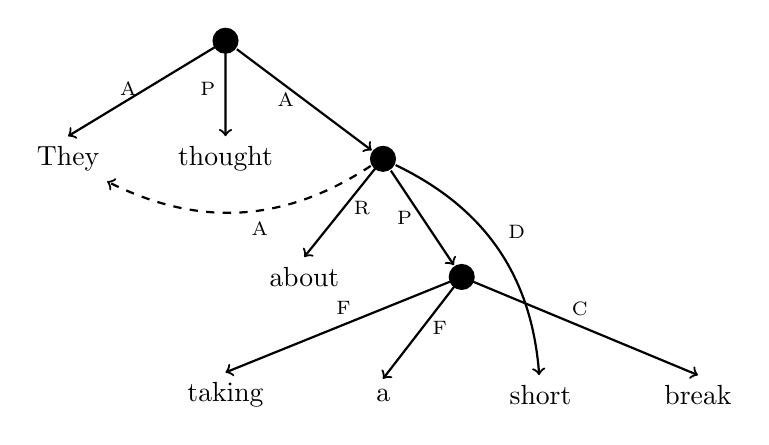
\begin{tikzpicture}[level distance=15mm, sibling distance=2cm, ->, thick,
    every node/.append style={font=\rmfamily},
    edge from parent/.append style={nodes={font=\scriptsize}},
    edge from parent path={(\tikzparentnode.center) -- (\tikzchildnode.north)}]
    \node(ROOT)[fill=black, circle] at (3,0) {}
      child {node (They) {They} edge from parent node [left] {A}}
      child {node (thought) {thought} edge from parent node [left] {P}}
      child {node (abouttakingashortbreak) [fill=black, circle] {} 
      { 
        child {node (to) {about} edge from parent node [right] {R}}
        child {node (takingabreak) [fill=black, circle] {}
        {
          child {node (take) {taking} edge from parent node [above] {F}}      
          child {node (a) {a} edge from parent node [right] {F}} 
          child {node (short) {short} edge from parent [draw=none]}
          child {node (break) {break} edge from parent node [above] {C}}  
        } edge from parent [draw=none]}
      } edge from parent [draw=none]}
      ;
    \draw(abouttakingashortbreak) to node [left] {\scriptsize P} (takingabreak); 
    \draw(ROOT) to node [left] {\scriptsize A} (abouttakingashortbreak);
    \draw[bend left,dashed] (abouttakingashortbreak) to node [auto] {\scriptsize A} (They);
    \draw[bend left] (abouttakingashortbreak) to node [auto] {\scriptsize D} (short);
\end{tikzpicture}
\caption{UCCA graph for the sentences
``They thought about taking a short break''.}\label{fig:theythoughtabouttakingashortbreak}
\end{figure}

The set of transitions implemented by TUPA is:

\{\textsc{Shift, Reduce, {Node$_X$}, Left-Edge$_X$, Right-Edge$_X$,}
\textsc{{Left-Remote$_X$}, {Right-Remote$_X$}, {Swap}, Finish}\}

These transitions enable {non-terminal nodes}, {reentrancy} and {discontinuity}.
To parse the sentence ``They thought about taking a short break'' (Figure~\ref{fig:theythoughtabouttakingashortbreak}),
an oracle parser would start from the initial state depicted in Figure~\ref{fig:initial_state},
and subsequently apply the following transition sequence:

\textsc{Shift}, \textsc{Right-Edge$_A$}, \textsc{Shift}, \textsc{Swap}, \textsc{Right-Edge$_P$}, \textsc{Reduce}, \textsc{Shift}, \textsc{Shift}, \textsc{Node$_R$}, \textsc{Reduce}, \textsc{Left-Remote$_A$}, \textsc{Shift}, \textsc{Shift}, \textsc{Node$_C$}, \textsc{Reduce}, \textsc{Shift}, \textsc{Right-Edge$_P$}, \textsc{Shift}, \textsc{Right-Edge$_F$}, \textsc{Reduce}, \textsc{Shift}, \textsc{Swap}, \textsc{Right-Edge$_D$}, \textsc{Reduce}, \textsc{Swap}, \textsc{Right-Edge$_A$}, \textsc{Reduce}, \textsc{Reduce}, \textsc{Shift}, \textsc{Reduce}, \textsc{Shift}, \textsc{Right-Edge$_C$}, \textsc{Finish}

\begin{figure}\centering
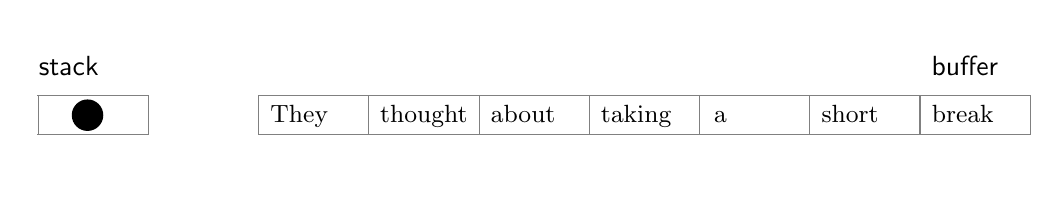
\begin{tikzpicture}[xscale=1.4,every node/.append style={font=\rmfamily,
                    anchor=west,text height=.6ex,text depth=0}, circle]
    \draw[xstep=1,ystep=.5,color=gray] (-.01,0) grid (1,.5);
    \node[style={font=\sffamily}] at (-.1,.8) {stack};
    \node[fill=black] at (.3,.25) {};
    \draw[xstep=1,ystep=.5,color=gray] (2,0) grid (9,.5);
    \node[style={font=\sffamily}] at (8,.8) {buffer};
    \node at (2,.2) {\small They};
    \node at (3,.2) {\small thought};
    \node at (4,.2) {\small about};
    \node at (5,.2) {\small taking};
    \node at (6,.2) {\small a};
    \node at (7,.2) {\small short};
    \node at (8,.2) {\small break};
\end{tikzpicture}
\caption{Initial state for parsing the sentence from Figure~\ref{fig:theythoughtabouttakingashortbreak}.}
\label{fig:initial_state}
\end{figure}

A few intermediate steps from this sequence are shown in Figure~\ref{fig:transition_sequence}.
Using supervised learning, TUPA would learn to mimic this oracle transition sequence
by training a neural network classifier with a cross-entropy loss
(see Section~\ref{sec:nn})
to produce the correct transition at each point in the transition sequence,
given the current state of the stack, the buffer and the graph.

\begin{figure}\centering
\begin{subfigure}{.45\textwidth}
Shift

\scalebox{.5}{
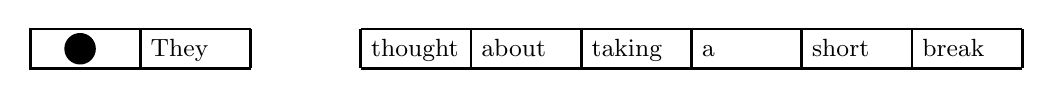
\begin{tikzpicture}[xscale=1.4,every node/.append style={font=\rmfamily, thick,
                    anchor=west,text height=.6ex,text depth=0}]
    \begin{scope}[xstep=1,ystep=.5,line width=1pt]
      \draw (.99, 0) grid (2,.5);
      \draw (-.01,0) grid (2, .5);
      \draw (3,   0) grid (9,.5);
    \end{scope}
    \node[fill=black, circle] at (.3, .25) {};
    \node at (1,.2) {\small They};
    \node at (3,.2) {\small thought};
    \node at (4,.2) {\small about};
    \node at (5,.2) {\small taking};
    \node at (6,.2) {\small a};
    \node at (7,.2) {\small short};
    \node at (8,.2) {\small break};
\end{tikzpicture}}
\fbox{\scalebox{.55}{
\begin{tikzpicture}[level distance=14mm, sibling distance=26mm, ->,
    every node/.append style={font=\rmfamily},
    edge from parent/.append style={nodes={font=\scriptsize}},
    edge from parent path={(\tikzparentnode.center) -- (\tikzchildnode.north)}]
    \node(ROOT)[fill=black, circle] at (3,0) {}
      child [draw=none] {node (They) {They} edge from parent [draw=none] node [left] {}}
      child [draw=none] {node (thought) {thought} edge from parent [draw=none] node [left] {}}
      child [draw=none] {node (abouttakingashortbreak) [draw=none] {}
      {
        child [draw=none] {node (to) {about} edge from parent [draw=none] node [right] {}}
        child [draw=none] {node (takingabreak) [draw=none] {}
        {
          child [draw=none] {node (take) {taking} edge from parent [draw=none] node [above] {}}
          child [draw=none] {node (a) {a} edge from parent [draw=none] node [right] {}}
          child [draw=none] {node (short) {short} edge from parent [draw=none]}
          child [draw=none] {node (break) {break} edge from parent [draw=none] node [above] {}}
        } edge from parent [draw=none]}
      } edge from parent [draw=none]}
      ;
\end{tikzpicture}}}
\end{subfigure}
\begin{subfigure}{.45\textwidth}
Right-Edge$_A$

\scalebox{.5}{
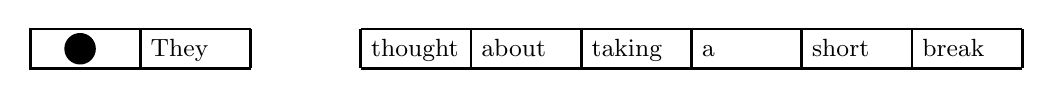
\begin{tikzpicture}[xscale=1.4,every node/.append style={font=\rmfamily, thick,
                    anchor=west,text height=.6ex,text depth=0}]
    \begin{scope}[xstep=1,ystep=.5,line width=1pt]
      \draw (-.01,0) grid (2,.5);
      \draw (-.01,0) grid (2, .5);
      \draw (3,   0) grid (9,.5);
    \end{scope}
    \node[fill=black, circle] at (.3, .25) {};
    \node at (1,.2) {\small They};
    \node at (3,.2) {\small thought};
    \node at (4,.2) {\small about};
    \node at (5,.2) {\small taking};
    \node at (6,.2) {\small a};
    \node at (7,.2) {\small short};
    \node at (8,.2) {\small break};
\end{tikzpicture}}
\fbox{\scalebox{.55}{
\begin{tikzpicture}[level distance=14mm, sibling distance=26mm, ->,
    every node/.append style={font=\rmfamily},
    edge from parent/.append style={nodes={font=\scriptsize}},
    edge from parent path={(\tikzparentnode.center) -- (\tikzchildnode.north)}]
    \node(ROOT)[fill=black, circle] at (3,0) {}
      child {node (They) {They} edge from parent node [left] {A}}
      child [draw=none] {node (thought) {thought} edge from parent [draw=none] node [left] {}}
      child [draw=none] {node (abouttakingashortbreak) [draw=none] {}
      {
        child [draw=none] {node (to) {about} edge from parent [draw=none] node [right] {}}
        child [draw=none] {node (takingabreak) [draw=none] {}
        {
          child [draw=none] {node (take) {taking} edge from parent [draw=none] node [above] {}}
          child [draw=none] {node (a) {a} edge from parent [draw=none] node [right] {}}
          child [draw=none] {node (short) {short} edge from parent [draw=none]}
          child [draw=none] {node (break) {break} edge from parent [draw=none] node [above] {}}
        } edge from parent [draw=none]}
      } edge from parent [draw=none]}
      ;
\end{tikzpicture}}}
\end{subfigure}

\begin{subfigure}{.45\textwidth}
Shift

\scalebox{.5}{
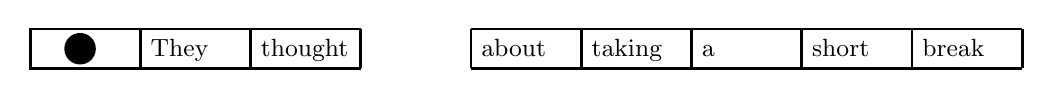
\begin{tikzpicture}[xscale=1.4,every node/.append style={font=\rmfamily, thick,
                    anchor=west,text height=.6ex,text depth=0}]
    \begin{scope}[xstep=1,ystep=.5,line width=1pt]
      \draw (1.99,0) grid (3,.5);
      \draw (-.01,0) grid (3, .5);
      \draw (4,   0) grid (9,.5);
    \end{scope}
    \node[fill=black, circle] at (.3, .25) {};
    \node at (1,.2) {\small They};
    \node at (2,.2) {\small thought};
    \node at (4,.2) {\small about};
    \node at (5,.2) {\small taking};
    \node at (6,.2) {\small a};
    \node at (7,.2) {\small short};
    \node at (8,.2) {\small break};
\end{tikzpicture}}
\fbox{\scalebox{.55}{
\begin{tikzpicture}[level distance=14mm, sibling distance=26mm, ->,
    every node/.append style={font=\rmfamily},
    edge from parent/.append style={nodes={font=\scriptsize}},
    edge from parent path={(\tikzparentnode.center) -- (\tikzchildnode.north)}]
    \node(ROOT)[fill=black, circle] at (3,0) {}
      child {node (They) {They} edge from parent node [left] {A}}
      child [draw=none] {node (thought) {thought} edge from parent [draw=none] node [left] {}}
      child [draw=none] {node (abouttakingashortbreak) [draw=none] {}
      {
        child [draw=none] {node (to) {about} edge from parent [draw=none] node [right] {}}
        child [draw=none] {node (takingabreak) [draw=none] {}
        {
          child [draw=none] {node (take) {taking} edge from parent [draw=none] node [above] {}}
          child [draw=none] {node (a) {a} edge from parent [draw=none] node [right] {}}
          child [draw=none] {node (short) {short} edge from parent [draw=none]}
          child [draw=none] {node (break) {break} edge from parent [draw=none] node [above] {}}
        } edge from parent [draw=none]}
      } edge from parent [draw=none]}
      ;
\end{tikzpicture}}}
\end{subfigure}
\begin{subfigure}{.45\textwidth}
Swap

\scalebox{.5}{
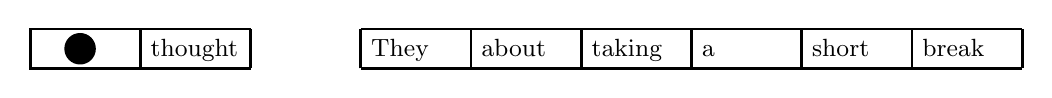
\begin{tikzpicture}[xscale=1.4,every node/.append style={font=\rmfamily, thick,
                    anchor=west,text height=.6ex,text depth=0}]
    \begin{scope}[xstep=1,ystep=.5,line width=1pt]
      \draw (3,   0) grid (4,.5);
      \draw (-.01,0) grid (2, .5);
      \draw (3,   0) grid (9,.5);
    \end{scope}
    \node[fill=black, circle] at (.3, .25) {};
    \node at (3,.2) {\small They};
    \node at (1,.2) {\small thought};
    \node at (4,.2) {\small about};
    \node at (5,.2) {\small taking};
    \node at (6,.2) {\small a};
    \node at (7,.2) {\small short};
    \node at (8,.2) {\small break};
\end{tikzpicture}}
\fbox{\scalebox{.55}{
\begin{tikzpicture}[level distance=14mm, sibling distance=26mm, ->,
    every node/.append style={font=\rmfamily},
    edge from parent/.append style={nodes={font=\scriptsize}},
    edge from parent path={(\tikzparentnode.center) -- (\tikzchildnode.north)}]
    \node(ROOT)[fill=black, circle] at (3,0) {}
      child {node (They) {They} edge from parent node [left] {A}}
      child [draw=none] {node (thought) {thought} edge from parent [draw=none] node [left] {}}
      child [draw=none] {node (abouttakingashortbreak) [draw=none] {}
      {
        child [draw=none] {node (to) {about} edge from parent [draw=none] node [right] {}}
        child [draw=none] {node (takingabreak) [draw=none] {}
        {
          child [draw=none] {node (take) {taking} edge from parent [draw=none] node [above] {}}
          child [draw=none] {node (a) {a} edge from parent [draw=none] node [right] {}}
          child [draw=none] {node (short) {short} edge from parent [draw=none]}
          child [draw=none] {node (break) {break} edge from parent [draw=none] node [above] {}}
        } edge from parent [draw=none]}
      } edge from parent [draw=none]}
      ;
\end{tikzpicture}}}
\end{subfigure}

\begin{subfigure}{.45\textwidth}
Right-Edge$_P$

\scalebox{.5}{
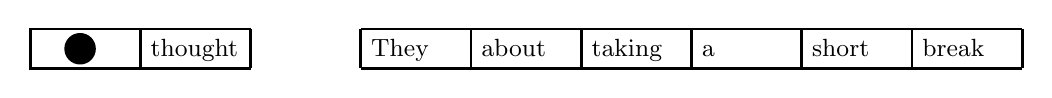
\begin{tikzpicture}[xscale=1.4,every node/.append style={font=\rmfamily, thick,
                    anchor=west,text height=.6ex,text depth=0}]
    \begin{scope}[xstep=1,ystep=.5,line width=1pt]
      \draw (-.01,0) grid (2,.5);
      \draw (-.01,0) grid (2, .5);
      \draw (3,   0) grid (9,.5);
      \draw (4,   0) grid (9,.5);
    \end{scope}
    \node[fill=black, circle] at (.3, .25) {};
    \node at (3,.2) {\small They};
    \node at (1,.2) {\small thought};
    \node at (4,.2) {\small about};
    \node at (5,.2) {\small taking};
    \node at (6,.2) {\small a};
    \node at (7,.2) {\small short};
    \node at (8,.2) {\small break};
\end{tikzpicture}}
\fbox{\scalebox{.55}{
\begin{tikzpicture}[level distance=14mm, sibling distance=26mm, ->,
    every node/.append style={font=\rmfamily},
    edge from parent/.append style={nodes={font=\scriptsize}},
    edge from parent path={(\tikzparentnode.center) -- (\tikzchildnode.north)}]
    \node(ROOT)[fill=black, circle] at (3,0) {}
      child {node (They) {They} edge from parent node [left] {A}}
      child {node (thought) {thought} edge from parent node [left] {}}
      child [draw=none] {node (abouttakingashortbreak) [draw=none] {}
      {
        child [draw=none] {node (to) {about} edge from parent [draw=none] node [right] {}}
        child [draw=none] {node (takingabreak) [draw=none] {}
        {
          child [draw=none] {node (take) {taking} edge from parent [draw=none] node [above] {}}
          child [draw=none] {node (a) {a} edge from parent [draw=none] node [right] {}}
          child [draw=none] {node (short) {short} edge from parent [draw=none]}
          child [draw=none] {node (break) {break} edge from parent [draw=none] node [above] {}}
        } edge from parent [draw=none]}
      } edge from parent [draw=none]}
      ;
\end{tikzpicture}}}
\end{subfigure}
\begin{subfigure}{.45\textwidth}
Reduce

\scalebox{.5}{
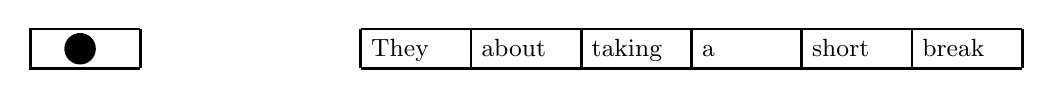
\begin{tikzpicture}[xscale=1.4,every node/.append style={font=\rmfamily, thick,
                    anchor=west,text height=.6ex,text depth=0}]
    \begin{scope}[xstep=1,ystep=.5,line width=1pt]
      \draw (-.01,0) grid (1, .5);
      \draw (3,   0) grid (9,.5);
      \draw (4,   0) grid (9,.5);
    \end{scope}
    \node[fill=black, circle] at (.3, .25) {};
    \node at (3,.2) {\small They};
    \node at (4,.2) {\small about};
    \node at (5,.2) {\small taking};
    \node at (6,.2) {\small a};
    \node at (7,.2) {\small short};
    \node at (8,.2) {\small break};
\end{tikzpicture}}
\fbox{\scalebox{.55}{
\begin{tikzpicture}[level distance=14mm, sibling distance=26mm, ->,
    every node/.append style={font=\rmfamily},
    edge from parent/.append style={nodes={font=\scriptsize}},
    edge from parent path={(\tikzparentnode.center) -- (\tikzchildnode.north)}]
    \node(ROOT)[fill=black, circle] at (3,0) {}
      child {node (They) {They} edge from parent node [left] {A}}
      child {node (thought) {thought} edge from parent node [left] {}}
      child [draw=none] {node (abouttakingashortbreak) [draw=none] {}
      {
        child [draw=none] {node (to) {about} edge from parent [draw=none] node [right] {}}
        child [draw=none] {node (takingabreak) [draw=none] {}
        {
          child [draw=none] {node (take) {taking} edge from parent [draw=none] node [above] {}}
          child [draw=none] {node (a) {a} edge from parent [draw=none] node [right] {}}
          child [draw=none] {node (short) {short} edge from parent [draw=none]}
          child [draw=none] {node (break) {break} edge from parent [draw=none] node [above] {}}
        } edge from parent [draw=none]}
      } edge from parent [draw=none]}
      ;
\end{tikzpicture}}}
\end{subfigure}
\caption{A few steps from a TUPA transition sequence.}\label{fig:transition_sequence}
\end{figure}

\section{Neural Networks}\label{sec:nn}

Neural networks are powerful machine learning models.
They have yielded state-of-the-art results in many fields,
including natural language processing \citep{goldberg2016primer}.
Inspired by the brain's computation mechanism,
artificial neural networks operate on dense input representations
by a combination of linear and non-linear transformations,
organized in several layers and trained end-to-end (\textit{deep learning}).
Deep learning and artificial neural networks have received much attention in
several fields of computer science, including computer vision, speech
recognition and natural language processing, due to their best performance in
various tasks \cite{collobert2011natural}.
In natural language processing, many of the deep learning methods rely strongly
on \textit{distributed representation}.

A common approach to meaning representation is the
representation of words as vectors in a continuous vector space with tens or
hundreds of dimensions \cite{turian2010word}, such that linguistic and semantic
regularities between the words are captured in the
vectors \cite{mikolov2013linguistic}. This kind of representation, called
\textit{word embedding}, can be learned in an unsupervised manner, from large
unlabeled corpora.
Several methods have been developed for generalizing these models to create embeddings
for multi-word phrases, sentences, and even complete documents.
These provides complementary semantic information about the text,
readily used in many machine learning techniques that operate on vectors of numbers.
The more accurately these vectors represent the meaning of the text, the better semantic tasks
can be solved using them.
However, composing these representation so as to maintain the semantic structure remains a challenge.

Language data is commonly manifested as sequences
(e.g., sentences are sequences of words).
Recurrent neural networks \citep{elman1990finding} allow representing
arbitrarily sized sequences in a fixed-size vector,
without ignoring the structured properties of the input.
A specific flavor called Long Short Term Memory
(LSTM) is very common as it learns relatively long-term dependencies.
A bidirectional recurrent neural network, such as a BiLSTM,
takes into account both the past and future
\cite{hochreiter1997long,schuster1997bidirectional,graves2008supervised,irsoy2014opinion}.

\textit{Recurrent} neural networks can learn semantically meaningful
continuous vector representations of multi-word phrases and sentences,
typically in the same space as the word embedding, and they have a relatively
simple model that does not depend on pre-annotation of structure:
the network \textit{state} at each time step is a function of the input and
the state at the previous time step:
\[
  h_t=f(x_t,h_{t-1})
\]
Where $f$ could be as simple as matrix multiplication followed by a non-linearity,
or a more complicated function such as an LSTM (Long-Short Term Memory) cell,
which supports additive gated updates for alleviating vanishing gradients:
\begin{align*}
    c_j =& c_{j-1} \odot f  + g\odot i \\
    h_j =& \tanh(c_j) \odot o            \\
    i =& \sigma(x_jW^{xi} + h_{j-1}W^{hi}) \\
    f =& \sigma(x_jW^{xf} + h_{j-1}W^{hf}) \\
    o =& \sigma(x_jW^{xo} + h_{j-1}W^{ho}) \\
    g =& \tanh(x_jW^{xg} + h_{j-1}W^{hg})
\end{align*}
A bidirectional LSTM (BiLSTM), or in general, a bidirectional recurrent neural network (BiRNN),
applies this function to the input sequence both in the original direction and
\textit{in reverse}, then concatenating the resulting hidden states for each position
in the sequence, and potentially applying the same operation again in multiple layers
(see Figure~\ref{fig:bilstm}).

\begin{figure}\centering
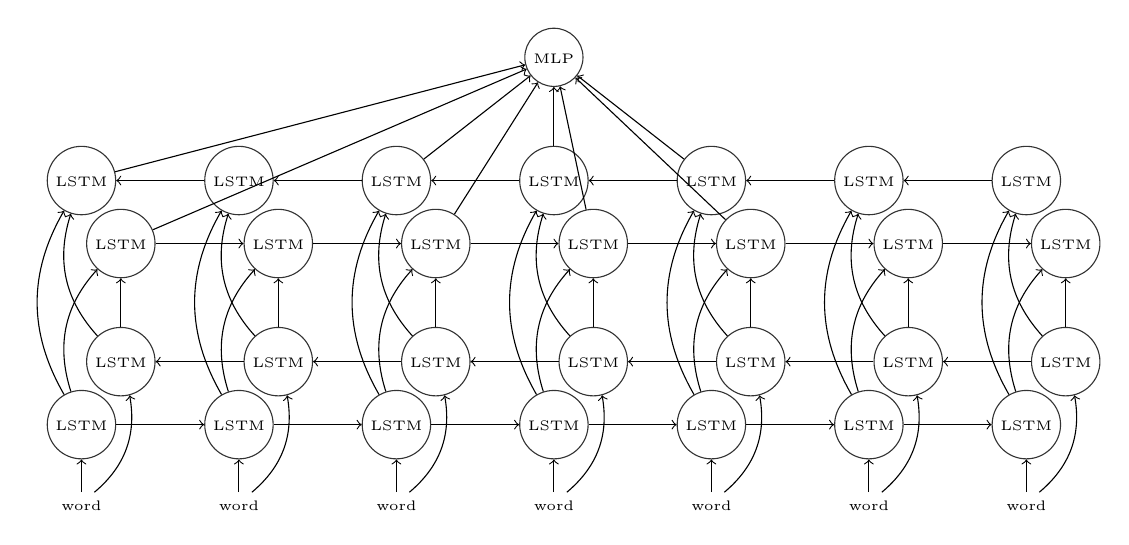
\begin{tikzpicture}[->,every node/.append style={anchor=north,text height=2ex,text depth=0}]
    \tiny
    \tikzstyle{main}=[circle, minimum size=7mm, draw=black!80, node distance=12mm]
    \foreach \i/\word in {1/{They},3/{thought},5/{about},7/{taking},9/{a},11/{short},13/{break}} {
        \node (x\i) at (\i,-1.3) {word};
        \node[main, fill=white!100] (h\i) at (\i,0) {LSTM};
        \path (x\i) edge (h\i);
        \node[main, fill=white!100] (i\i) at (\i.5,.8) {LSTM};
        \path (x\i) edge [bend right] (i\i);
        \node[main, fill=white!100] (l\i) at (\i.5,2.3) {LSTM};
        \path (h\i) edge [bend left] (l\i);
        \path (i\i) edge (l\i);
        \node[main, fill=white!100] (k\i) at (\i,3.1) {LSTM};
        \path (i\i) edge [bend left] (k\i);
        \path (h\i) edge [bend left] (k\i);
    }
    \foreach \current/\next in {1/3,3/5,5/7,7/9,9/11,11/13} {
        \path (h\current) edge (h\next);
        \path (i\next) edge (i\current);
        \path (l\current) edge (l\next);
        \path (k\next) edge (k\current);
    }
    \node[main, fill=white!100] (mlp) at (7,4.6) {MLP};
    \foreach \i in {1,5,7,9} {
        \path (l\i) edge (mlp);
        \path (k\i) edge (mlp);
    }
\end{tikzpicture}
\caption{BiLSTM encoder with MLP classifier.}\label{fig:bilstm}
\end{figure}

Typically, a feedforward neural network (MLP; multilayer perceptron) is applied on top
of these representations, and a \textit{softmax} classifier defines a probability
distribution based on the scores for each label:
\[[softmax(x)]_i = \frac{e^{x_i}}{\sum_je^{x_j}}\]

\textit{Recursive} neural networks can also learn phrase representations, taking advantage
of a pre-annotated hierarchical representation (typically syntactic trees) for
compositionality \cite{socher2010learning}.
These models can learn a representation that facilitates reasoning and inference \cite{bowman2014recursive}.
A recursive neural network has a state at each node of the structure: if $C_i$ denotes the set of children of
node $i$,
\[
  h_i=g(\{f(c)\;|\;c\in C_i\})
\]
where $g$ is an aggregation function, such as concatenation, addition or $\mathrm{max}$.
It can also be a variant of the LSTM cell \cite{tai-etal-2015-improved}.

A recursive neural network can also be used for structure prediction, or parsing
\cite{socher2013recursive,dyer2015transition}: as the parse is being created, the model can
be used to calculate the intermediate representation at each of the nodes already constructed,
and to make subsequent parsing decisions based upon it.
However, doing so efficiently requires specialized data structures \cite{bowman2016fast},
and is not suitable for predicting complex structures such as UCCA graphs.

\begin{figure}[ht!]\small
  \begin{subfigure}{\textwidth}
  \parbox{.2\textwidth}{\caption{}\label{fig:rnn}}
  \parbox{.8\textwidth}{
  \centering
  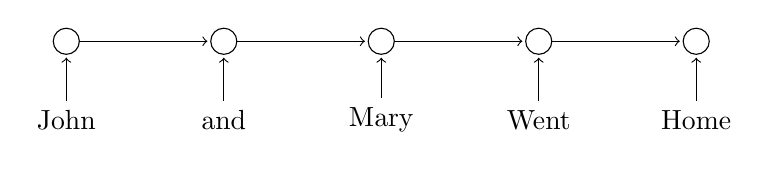
\begin{tikzpicture}[shorten >=1pt,->]
  \tikzstyle{vertex}=[circle,draw=black]
  \foreach \name/\x in {John/1, and/3, Mary/5, Went/7, Home/9}{
    \node[vertex] (G-\name) at (\x,1) {};
    \node (\name) at (\x,0) {\name};
    \draw (\name) -- (G-\name);
  }
  \foreach \from/\to in {John/and,and/Mary,Mary/Went,Went/Home}
    \draw (G-\from) -- (G-\to);
  \end{tikzpicture}
  }
  \end{subfigure}
  \begin{subfigure}{\textwidth}
  \parbox{.2\textwidth}{\caption{}\label{fig:recnn}}
  \parbox{.8\textwidth}{
  \centering
  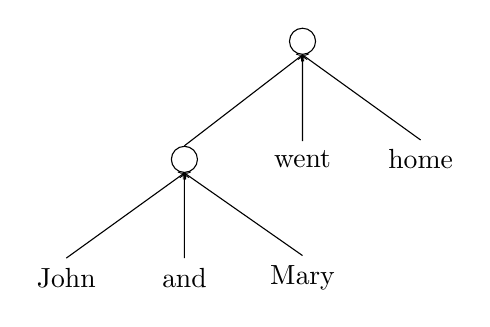
\begin{tikzpicture}[<-]
  \tikzstyle{vertex}=[circle,draw=black]
  \node[vertex] {}
    child {node [vertex] {}
    {
      child {node {John} edge from parent node[] {}}
      child {node {and} edge from parent node[] {}}
      child {node {Mary} edge from parent node[] {}}
    } edge from parent node[] {}}
    child {node {went} edge from parent node[] {}}
    child {node {home} edge from parent node[] {}}
    ;
  \end{tikzpicture}
  }
  \end{subfigure}
  \caption{\label{fig:nns}
    A recurrent neural network (a) combines distributed representations along a
    linear structure, whereas a recursive neural network (b) does so along a
    pre-determined hierarchical structure.
  }
\end{figure}
Neural networks are typically trained by gradient descent, where the gradient for the network parameters
is calculated using backpropagation.
The gradients for training a recursive neural network are calculated by \textit{backpropagation
through structure}, another variant of backpropagation, using a recursive
``folding'' architecture that can represent a general tree or a directed acyclic
graph (DAG) structure \cite{goller1996learning}.

Training neural predictors for independent or sequential predictions is often done
with the categorical cross-entropy loss (also referred to as \emph{negative log
likelihood}):
\begin{align*}
    L(\hat{y},y) = -\sum_i y_i\log(\hat{y}_i)
\end{align*}
It measures the dissimilarity between the true label distribution
$y$ and the predicted label distribution $\hat{y}$.
This is the loss function we use for training the transition classifier in TUPA,
given oracle transitions from an input gold graph.

Neural networks-based \textit{machine translation} provides some sort of
an intermediate encoding in the form of distributed representation that can be
encoded from the source language and then decoded into the target
language \cite{zou2013bilingual}, or using memory and treating the text as a
sequence to be converted to another sequence \cite{sutskever2014sequence},
using the popular sequence-to-sequence approach.
However, the encoding is based just on averaging across words in the source
sentence, on a flat sequence representation, or at best on a syntactic
representation. A semantic representation like a UCCA graph would perhaps be a
better candidate for the structure by which the encoding and decoding is
performed.

While for simple classification tasks such as Textual Entailment or
Natural Language Inference \cite{dagan2005pascal,snli:emnlp2015},
and to some degree for tasks with a complex output, such as machine translation, too,
simple end-to-end neural networks can go a long way \cite[among others]{bowman2015tree},
combinatorical generalization in learning inevitably requires an inductive bias
on the hypothesis class, realized as the network architecture
\cite{mitchell1980need,battaglia2018relational}.
Specifically, scalable learning of meaning and inference requires an inductive bias
on the compositional structure of language.


  \begin{center}
    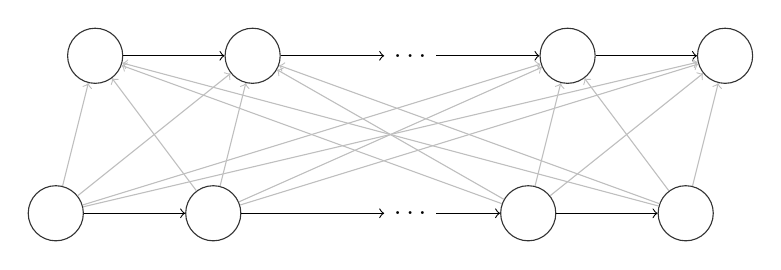
\begin{tikzpicture}[->]
    \tikzstyle{main}=[circle, minimum size=7mm, draw=black!80, node distance=12mm]
    \foreach \i in {1,3,7,9} {
        \node[main, fill=white!100] (h\i) at (\i,0) {};
        \node[main, fill=white!100] (o\i) at (\i.5,2) {};
    }
    \node (h5) at (5.5,0) {$\ldots$};
    \node (o5) at (5.5,2) {$\ldots$};
    \foreach \current/\next in {1/3,3/5,5/7,7/9} {
        \path (h\current) edge (h\next);
        \path (o\current) edge (o\next);
    }
    \foreach \i in {1,3,7,9} {
      \foreach \j in {1,3,7,9} {
        \path[gray!50] (h\i) edge (o\j);
      }
    }
    \end{tikzpicture}
  \end{center}

Perhaps just as critical as the successful prediction of UCCA structure, if not
even more critical for the NLP community, is the distributed representation
created when forming phrases using this structure. Current methods in NLP form
multi-word representation based on averaging across words or on syntax, which
may be sub-optimal in representing the true meaning of text. Using a more
semantically faithful way to compose words, such as UCCA, may be a key factor
in enabling computers to understand natural language.


\section{Multitask Learning}\label{sec:multitask}

Multitask learning \citep{caruana1998multitask} allows exploiting the overlap between tasks
to effectively extend the training data, 
and has greatly advanced with neural networks and representation learning.
It has been used over the years for NLP tasks with varying degrees of similarity.
Joint and multitask learning are often used
when two or more tasks share common information.
These techniques have been used in NLP with tasks of varying degrees of similarity---as
regularization, or to enlarge the effective training data.

In semantic role labeling, \citet{toutanova2005joint}
learned a joint re-reranking log-linear model across arguments of the same predicate.
\citet{Q16-1031,guo2016exploiting} applied multitask learning to transition-based
syntactic parsing in a multilingual setting.
Joint learning is also often used
as an alternative to the pipeline approach, alleviating error propagation:
In transition-based parsing, multitask learning has also been applied to
tagging and parsing \cite{bohnet2012transition,Zhang2016StackpropagationIR},
lexical and syntactic analysis \cite{constant-nivre:2016:P16-1,more2016joint},
and semantic-syntactic analysis \cite{swayamdipta-EtAl:2016:CoNLL,henderson2013multilingual}.

Neural multitask learning has mostly been effective in tackling formally similar
tasks \citep{P16-2038},
including multilingual semantic parsing \citep{duong2017multilingual},
and cross-domain semantic parsing \citep{herzig-berant:2017:Short,W17-2607}.
Sharing parameters with a low-level task
has shown great benefit for transition-based syntactic parsing
\citep{bohnet2012transition,Zhang2016StackpropagationIR,constant-nivre:2016:P16-1,more2016joint}.
State-of-the-art results in multiple NLP tasks have been achieved
by jointly learning the tasks forming the NLP standard pipeline using 
a single neural model \citep{collobert2011natural,D17-1206},
thereby avoiding cascading errors, common in pipelines.

Much effort has been devoted to joint learning of syntactic
and semantic parsing, including
two CoNLL shared tasks \cite{surdeanu2008conll,hajivc2009conll}
on joint syntactic parsing and semantic role labeling.
Despite their conceptual and practical appeal, such joint models rarely outperform
the pipeline approach of basing semantic parsing on the output of syntactic parsers
\cite{lluis2008joint,henderson2013multilingual,D15-1169,swayamdipta-EtAl:2016:CoNLL,swayamdipta2017frame}.

This thesis revisits the idea of multitask learning for transition-based parsing
with neural networks, combining an unprecedented diverse set of semantic parsing
tasks and learning them with a uniform model.
While many multitask architectures exist and have different advantages,
the approach taken here is hard parameter sharing in the encoder layers of a neural
network used for classification.

\section{Evaluation}
Comparing UCCA structures
$G_p=(V_p,E_p,\ell_p)$ and $G_g=(V_g,E_g,\ell_g)$,
over the same sequence of terminals $W = \{w_1,\ldots,w_n\}$
is done as follows.
For an edge $e=(u,v)$ in either graph, its yield $y(e) \subseteq W$ is the
set of terminals in $W$ that are descendants of $v$.
Define the set of \textit{mutual edges} between $G_p$ and $G_g$:
\[
    M(G_p,G_g) =
    \left\{(e_1,e_2) \in E_p \times E_g \;|\;
    y(e_1) = y(e_2) \wedge \ell_p(e_1)=\ell_g(e_2)\right\}
\]

Labeled precision and recall are defined by dividing $|M(G_p,G_g)|$ by $|E_p|$ and $|E_g|$, respectively,
and F-score by taking their harmonic mean.
Two variants are reported: one where we consider only primary edges,
and another for remote edges.
In all cases, punctuation units (U) are excluded from the evaluation.


\include{acl2017}
\include{acl2018}
\include{udst2018}
\include{divergences}


\chapter{Discussion}

In this thesis, I showed that meaning representation is valuable for language understanding,
and that TUPA, an accurate UCCA parser, is suited to many meaning representations.
Furthermore, multitask learning allows useful shared generalizations to emerge,
improving TUPA's performance by taking advantage of its general transition-based
architecture and flexible neural network classifier.
As different meaning representations capture many similar distinctions,
this approach proved effective, gaining from data annotated in each scheme
even though they had been designed separately and with different formal properties.
While divergences between the content of the schemes may limit the gain from sharing,
they highlight relative strengths, which are meaningful both theoretically and practically.

\section{Objectives}

The objective of this thesis (see Section~\ref{sec:intro_ucca_parsing}) were to
develop techniques for graph parsing in general and UCCA in particular,
comparing UCCA to other representation schemes,
and hybridizing meaning representations and parsers to improve their performance.
Indeed, in Chapter~\ref{acl2017}, an accurate and efficient UCCA parser was presented,
and in Chapter~\ref{udst2018} its applicability was demonstrated to Universal Dependencies.
In Chapter~\ref{acl2018} more representation frameworks were shown to be supported by
the parser, and furthermore, transfer and multitask learning were shown to effectively
improve parsing performance by taking advantage of shared generalizations.
Finally, Chapter~\ref{divergences} provided a thorough qualitative and quantitative
analysis of UCCA and Universal Dependencies, highlighting the content differences,
the semantic divergences and points of similarity.

UCCA's merits in providing a cross-linguistically applicable,
broad-coverage annotation will support ongoing efforts to incorporate deeper
semantic structures into a variety of applications, such as machine translation
\citep{jones2012semantics} and summarization \citep{liu2015toward}.
The advantage of UCCA as compared to syntactic annotation schemes for machine translation is apparent,
as translation tends to preserve semantic structure more than syntactic structure \citep{sulem2015conceptual}.
Using UCCA as an intermediate representation is thus likely to achieve outputs that are more
semantically similar to the source.

\section{Challenges}

At the initial stages of this work, dataset size was a concern.
Models with a large number of parameters,
such as the neural network models employed in TUPA,
typically require very large training sets.
Since the UCCA datasets are small in relation to other schemes,
training neural network models on them seemed to pose a challenge.
However,
the current performance of TUPA in UCCA parsing is already quite satisfactory.
This is demonstrated by the fact that the parser has been successfully used in
various applications \cite{choshen2018reference,sulem2018semantic,sulem2018simple}.
Furthermore,
multitask learning proved to be an effective method to overcome the data scarcity issue.
The UCCA data has also been slowly growing and extended to more languages by further labeling efforts,
and results seem to improve as more and more training data is available.

While many distinctions are shared between UCCA and other semantic and syntactic schemes,
they are largely obscured by differences in representation format and convention.
A second challenge was thus in developing a generic parsing system that would be able
to handle more than one semantic scheme.
However, the general architecture of the parser was effective in handling these
graphs structure.
Conversion to a common graph format and assimilation of superficial structures
addressed the generality question effectively to allow multitask learning,
and further, allowed deep inspection of content divergences and convergences.

\section{Further Analysis}

\subsection{Benefit of Multitask Learning}

To further quantify the improvements due to multitask learning, where the tasks of parsing
multiple semantic representations are combined as auxiliary tasks for TUPA to improve UCCA
parsing, Figure~\ref{fig:fine_grained} offers a fine-grained analysis of the performance of different
multitask models.
The benefit of the multitask models over the single-task baseline is especially apparent for
Connectors and Linkers, demonstrating the improved capability to parse coordination structures
correctly, which are indeed relevant for all meaning representations.
Furthermore, while the labeled F1 for State is uniformly low due to the rarity of this category
and its common confusion with Process, the multitask model with all auxiliary task is able to reach
40\% labeled F1, showing it is able to generalize this difficult distinction between predicates
describing events and attributes.
In French and German, the improvement is again apparent for Connectors and Linkers,
but now especially also for Parallel Scenes---these seem to be responsible for most of the improvement
due to multitask learning in these languages.
Again, this shows that the syntactic ability to split phrases and clauses to separate Scenes is greatly
boosted by the auxiliary task (UD in this case).

Figure~\ref{fig:fine_grained_ud} shows fine-grained analysis by UD relations.
Surprisingly, determiners seem to suffer from multitask learning, as the single-task baseline does
best on them.
While determiners in UCCA are mostly Elaborators (in the version of the corpora on which the experiment
was made), they are mostly treated as vacuous semantically in DM and AMR, which could explain their
poor representation in models trained with these auxiliary tasks.
UD as an auxiliary greatly helps with this category in French and German, but also seems to deteriorate
its treatment in English.
Prepositions in German (bearing the case relation) are greatly improved by adding UD as an auxiliary.
This is a common relation, spread over multiple UCCA categories. Learning to represent it more accurately
improves performance across the board.


\pgfplotstableread{
category	single	UCCAAMR	UCCAUD	UCCADM	UCCADMUD	UCCAAMRUD	UCCAAMRDM	UCCAAMRDMUD
Participant	77	76	77	77	77	77	77	78
Center	78	77	77	78	80	78	79	79
Adverbial	78	75	77	77	75	76	75	75
Elaborator	77	77	77	78	78	79	79	78
ParallelScene	75	76	75	78	77	75	77	76
Connector	83	84	84	86	89	84	90	87
Relator	92	91	91	92	93	92	92	92
State	35	37	36	38	37	36	34	40
Function	82	82	80	83	84	85	83	84
Process	78	77	76	76	78	77	78	77
Linker	78	84	82	87	81	82	82	83
}\englishwiki
\pgfplotstableread{
category	single	UCCAUD
Participant	38	48
Center	77	76
Adverbial	25	32
Elaborator	21	26
ParallelScene	23	38
Connector	78	89
Relator	16	14
State	0	0
Function	67	68
Process	0	0
Linker	30	50
}\french
\pgfplotstableread{
category	single	UCCAUD
Participant	79	84
Center	89	90
Adverbial	66	72
Elaborator	87	89
ParallelScene	41	83
Connector	78	86
Relator	79	80
State	93	93
Function	0	0
Process	88	85
Linker	71	72
}\german


\pgfplotstableread{
category	single	UCCAAMR	UCCAUD	UCCADM	UCCADMUD	UCCAAMRUD	UCCAAMRDM	UCCAAMRDMUD
case	84	82	84	82	85	83	82	83
compound	83	84	87	81	83	81	81	78
iobj	85	82	83	84	82	83	84	86
nmod	85	84	85	86	88	85	84	87
nsubj	78	78	77	77	83	81	82	81
obj	88	84	84	88	93	87	86	91
appos	84	83	86	85	85	85	83	85
conj	76	80	78	81	80	81	80	81
det	82	67	59	53	67	67	47	57
acl	80	81	82	83	81	80	83	81
amod	81	83	86	86	86	84	86	83
}\englishwikiud
\pgfplotstableread{
category	single	UCCAAMR	UCCAUD	UCCADM	UCCADMUD	UCCAAMRUD	UCCAAMRDM	UCCAAMRDMUD
aux	84	83	83	85	86	84	84	86
obl	78	77	78	80	79	79	83	80
advcl	81	78	81	79	82	82	82	80
expl	64	65	60	63	62	62	59	69
mark	44	44	44	50	44	50	44	50
cc	80	93	80	93	93	93	93	93
advmod	83	83	82	86	84	85	85	83
nummod	84	90	94	87	81	90	84	94
ccomp	86	86	86	86	86	86	86	86
}\englishwikiudb
\pgfplotstableread{
category	single	UCCAUD
case	78	84
compound	22	32
iobj	10	18
nmod	34	51
nsubj	27	34
obj	19	38
appos	37	17
conj	26	31
det	87	89
acl	11	23
amod	48	51
aux	47	70
obl	27	41
advcl	13	14
expl	12	12
mark	29	36
cc	42	64
advmod	19	26
nummod	58	44
parataxis	0	27
cop	44	28
ccomp	10	41
xcomp	22	28
}\frenchud
\pgfplotstableread{
category	single	UCCAUD
case	6	82
compound	74	79
iobj	59	67
nmod	90	91
nsubj	95	96
obj	84	85
appos	89	92
conj	79	81
det	10	91
acl	65	72
amod	80	90
aux	62	63
obl	45	73
advcl	75	79
expl	74	76
mark	76	76
cc	73	76
advmod	53	62
nummod	76	74
parataxis	78	90
cop	90	91
ccomp	56	79
xcomp	67	67
}\germanud

\begin{figure}
\begin{subfigure}{\textwidth}
    \begin{tikzpicture}
    \begin{axis}[
    ybar=0pt,
    ymin=0,
    width=17cm,
    height=6cm,
    bar width=4pt,
    xtick=data,
    xticklabels from table={\englishwiki}{category},
    xticklabel style={font=\tiny,rotate=50,anchor=east},
    xtick align=inside,
    xticklabel pos=left,
    yticklabels=none,
    tickwidth=0pt,
    legend style={at={(axis cs:-1,100)},anchor=south west,font=\tiny,draw=none,legend columns=-1},
    legend cell align={left},
    nodes near coords={\scalebox{.4}{\pgfmathprintnumber[precision=2]{\pgfplotspointmeta}}},
    every node near coord/.append style={rotate=90,anchor=west}]
    \addplot[fill=green]table[x expr=\coordindex,meta=category,y=single]{\englishwiki};
    \addplot[fill=blue]table[x expr=\coordindex,meta=category,y=UCCAAMR]{\englishwiki};
    \addplot[fill=red]table[x expr=\coordindex,meta=category,y=UCCAUD]{\englishwiki};
    \addplot[fill=orange]table[x expr=\coordindex,meta=category,y=UCCADM]{\englishwiki};
    \addplot[fill=magenta]table[x expr=\coordindex,meta=category,y=UCCADMUD]{\englishwiki};
    \addplot[fill=cyan]table[x expr=\coordindex,meta=category,y=UCCAAMRUD]{\englishwiki};
    \addplot[fill=yellow]table[x expr=\coordindex,meta=category,y=UCCAAMRDM]{\englishwiki};
    \addplot[fill=brown]table[x expr=\coordindex,meta=category,y=UCCAAMRDMUD]{\englishwiki};
    \legend{Single,UCCA+AMR,UCCA+UD,UCCA+DM,UCCA+DM+UD,UCCA+AMR+UD,UCCA+AMR+DM,All}
    \end{axis}
    \end{tikzpicture}
    \caption{English Wiki}
\end{subfigure}
\begin{subfigure}{.475\textwidth}
    \begin{tikzpicture}
    \begin{axis}[
    ybar=0pt,
    ymin=0,
    width=9cm,
    height=6cm,
    bar width=4pt,
    xtick=data,
    xticklabels from table={\french}{category},
    xticklabel style={font=\tiny,rotate=50,anchor=east},
    xtick align=inside,
    xticklabel pos=left,
    yticklabels=none,
    tickwidth=0pt,
    nodes near coords={\scalebox{.4}{\pgfmathprintnumber[precision=2]{\pgfplotspointmeta}}},
    every node near coord/.append style={rotate=90,anchor=west}]
    \addplot[fill=green]table[x expr=\coordindex,meta=category,y=single]{\french};
    \addplot[fill=red]table[x expr=\coordindex,meta=category,y=UCCAUD]{\french};
    \end{axis}
    \end{tikzpicture}
    \caption{French 20K}
\end{subfigure}
\begin{subfigure}{.475\textwidth}
    \begin{tikzpicture}
    \begin{axis}[
    ybar=0pt,
    ymin=0,
    width=9cm,
    height=6cm,
    bar width=4pt,
    xtick=data,
    xticklabels from table={\german}{category},
    xticklabel style={font=\tiny,rotate=50,anchor=east},
    xtick align=inside,
    xticklabel pos=left,
    yticklabels=none,
    tickwidth=0pt,
    nodes near coords={\scalebox{.4}{\pgfmathprintnumber[precision=2]{\pgfplotspointmeta}}},
    every node near coord/.append style={rotate=90,anchor=west}]
    \addplot[fill=green]table[x expr=\coordindex,meta=category,y=single]{\german};
    \addplot[fill=red]table[x expr=\coordindex,meta=category,y=UCCAUD]{\german};
    \end{axis}
    \end{tikzpicture}
    \caption{German 20K}
\end{subfigure}
    \caption{TUPA's F1 per UCCA category in each single-/multitask setting.
    \label{fig:fine_grained}}
\end{figure}

\begin{figure}
\begin{subfigure}{\textwidth}
    \begin{tikzpicture}
    \begin{axis}[
    ybar=0pt,
    ymin=0,
    width=17cm,
    height=5cm,
    bar width=4pt,
    xtick=data,
    xticklabels from table={\englishwikiud}{category},
    xticklabel style={font=\tiny,rotate=50,anchor=east},
    xtick align=inside,
    xticklabel pos=left,
    yticklabels=none,
    tickwidth=0pt,
    legend style={at={(axis cs:-1,100)},anchor=south west,font=\tiny,draw=none,legend columns=-1},
    legend cell align={left},
    nodes near coords={\scalebox{.4}{\pgfmathprintnumber[precision=2]{\pgfplotspointmeta}}},
    every node near coord/.append style={rotate=90,anchor=west}]
    \addplot[fill=green]table[x expr=\coordindex,meta=category,y=single]{\englishwikiud};
    \addplot[fill=blue]table[x expr=\coordindex,meta=category,y=UCCAAMR]{\englishwikiud};
    \addplot[fill=red]table[x expr=\coordindex,meta=category,y=UCCAUD]{\englishwikiud};
    \addplot[fill=orange]table[x expr=\coordindex,meta=category,y=UCCADM]{\englishwikiud};
    \addplot[fill=magenta]table[x expr=\coordindex,meta=category,y=UCCADMUD]{\englishwikiud};
    \addplot[fill=cyan]table[x expr=\coordindex,meta=category,y=UCCAAMRUD]{\englishwikiud};
    \addplot[fill=yellow]table[x expr=\coordindex,meta=category,y=UCCAAMRDM]{\englishwikiud};
    \addplot[fill=brown]table[x expr=\coordindex,meta=category,y=UCCAAMRDMUD]{\englishwikiud};
    \legend{Single,UCCA+AMR,UCCA+UD,UCCA+DM,UCCA+DM+UD,UCCA+AMR+UD,UCCA+AMR+DM,All}
    \end{axis}
    \end{tikzpicture}
    \caption{English Wiki}
\end{subfigure}
\begin{subfigure}{\textwidth}
    \begin{tikzpicture}
    \begin{axis}[
    ybar=0pt,
    ymin=0,
    width=17cm,
    height=5cm,
    bar width=4pt,
    xtick=data,
    xticklabels from table={\englishwikiudb}{category},
    xticklabel style={font=\tiny,rotate=50,anchor=east},
    xtick align=inside,
    xticklabel pos=left,
    yticklabels=none,
    tickwidth=0pt,
    nodes near coords={\scalebox{.4}{\pgfmathprintnumber[precision=2]{\pgfplotspointmeta}}},
    every node near coord/.append style={rotate=90,anchor=west}]
    \addplot[fill=green]table[x expr=\coordindex,meta=category,y=single]{\englishwikiudb};
    \addplot[fill=blue]table[x expr=\coordindex,meta=category,y=UCCAAMR]{\englishwikiudb};
    \addplot[fill=red]table[x expr=\coordindex,meta=category,y=UCCAUD]{\englishwikiudb};
    \addplot[fill=orange]table[x expr=\coordindex,meta=category,y=UCCADM]{\englishwikiudb};
    \addplot[fill=magenta]table[x expr=\coordindex,meta=category,y=UCCADMUD]{\englishwikiudb};
    \addplot[fill=cyan]table[x expr=\coordindex,meta=category,y=UCCAAMRUD]{\englishwikiudb};
    \addplot[fill=yellow]table[x expr=\coordindex,meta=category,y=UCCAAMRDM]{\englishwikiudb};
    \addplot[fill=brown]table[x expr=\coordindex,meta=category,y=UCCAAMRDMUD]{\englishwikiudb};
    \end{axis}
    \end{tikzpicture}
    \caption{English Wiki (cont.)}
\end{subfigure}
\begin{subfigure}{\textwidth}
    \begin{tikzpicture}
    \begin{axis}[
    ybar=0pt,
    ymin=0,
    width=17cm,
    height=5cm,
    bar width=4pt,
    xtick=data,
    xticklabels from table={\frenchud}{category},
    xticklabel style={font=\tiny,rotate=50,anchor=east},
    xtick align=inside,
    xticklabel pos=left,
    yticklabels=none,
    tickwidth=0pt,
    nodes near coords={\scalebox{.4}{\pgfmathprintnumber[precision=2]{\pgfplotspointmeta}}},
    every node near coord/.append style={rotate=90,anchor=west}]
    \addplot[fill=green]table[x expr=\coordindex,meta=category,y=single]{\frenchud};
    \addplot[fill=red]table[x expr=\coordindex,meta=category,y=UCCAUD]{\frenchud};
    \end{axis}
    \end{tikzpicture}
    \caption{French 20K}
\end{subfigure}
\begin{subfigure}{\textwidth}
    \begin{tikzpicture}
    \begin{axis}[
    ybar=0pt,
    ymin=0,
    width=17cm,
    height=5cm,
    bar width=4pt,
    xtick=data,
    xticklabels from table={\germanud}{category},
    xticklabel style={font=\tiny,rotate=50,anchor=east},
    xtick align=inside,
    xticklabel pos=left,
    yticklabels=none,
    tickwidth=0pt,
    nodes near coords={\scalebox{.4}{\pgfmathprintnumber[precision=2]{\pgfplotspointmeta}}},
    every node near coord/.append style={rotate=90,anchor=west}]
    \addplot[fill=green]table[x expr=\coordindex,meta=category,y=single]{\germanud};
    \addplot[fill=red]table[x expr=\coordindex,meta=category,y=UCCAUD]{\germanud};
    \end{axis}
    \end{tikzpicture}
    \caption{German 20K}
\end{subfigure}
    \caption{TUPA's F1 per UD relation in each single-/multitask setting.
    \label{fig:fine_grained_ud}}
\end{figure}


\section{Ongoing Work}

The ideas presented in this thesis offer many exciting opportunities for further research.
Following are such directions, which I have started pursuing.

\subsection{Combining Syntax with Lexical Semantics}

In the comparison between Universal Dependencies (UD) and UCCA,
88\% of edges were found to be common between the schemes (ignoring the label),
meaning the linguistic structures annotated by them are very similar.
Inspecting the remaining divergences reveals, for example, that only
about 82\% of UCCA unanalyzable units (i.e., units without a compositional
internal structure) are even sub-trees in UD.
The remaining cases seem to be almost exclusively multi-word Linkers,
such as ``even though'', ``when it comes to'' and ``just because''.
Furthermore, only 73\% of Participants in UCCA Scenes were found to be arguments
of syntactic predicates in UD, due to the differences in distinctions between
Scenes/non-Scenes and between main relations, secondary relations and participants.

These gaps can perhaps be closed
by complementing syntax with \textit{lexical} semantics to make up for differences
corresponding to semantic distinctions that are not expressed in UD.
Lexical semantic resources, such as STREUSLE
\citep{schneider-thesis,envmwe,pssdisambig,gensuper},
may provide the necessary annotation to close the gap between UD and UCCA:
for example, it contains labels for various types of multi-word expressions,
even ones that are not UD sub-trees;
and semantically categorize lexical items according to lexical category and
supersense, distinguishing, for example, eventive from non-eventive nouns.
This will also address the need for a comparison of UD \textit{enhanced dependencies}
and UCCA remote and implicit units, mentioned in Chapter~\ref{divergences}.

\subsection{Broad-coverage Semantic Parsing}

While implicit units (see Section~\ref{sec:intro_ucca}) are not supported
by the original parser presented in Chapter~\ref{acl2017},
ongoing work, beyond the scope of this thesis, addresses
the prediction of implicit arguments in UCCA and other meaning representations
\cite{bender2011parser,cheng2018implicit,petruck2019meaning}
with a general mechanism that can be used to augment a UCCA parser
to support implicit unit prediction.
Similarly, the phenomenon of elided predicates and null nodes in Universal Dependencies,
mentioned in Chapter~\ref{udst2018}, overlaps with the phenomenon of implicit units
(where in this case the main relation is implicit rather than an argument),
and can be addressed by a similar technique.

\subsection{Establishing the Meaning Representation Parsing Task}

TUPA, the parser presented in this thesis, is the first UCCA parser.
In other parsing tasks, years of experiments and progress have yielded very
accurate and fine-tuned parsers.
While TUPA is quite accurate, there can doubtlessly be countless improvements
due to different ways of looking at the problem or a better selection of architecture
and parameters.
During January 2019, we (Zohar Aizenbud, Leshem Choshen, Elior Sulem, Omri Abend,
Ari Rappoport and myself) ran a shared task as part of the
International Workshop on Semantic Evaluation, titled
Task 1: Cross-lingual Semantic Parsing with UCCA.
The task presented participants with UCCA parsing challenges
in English, German and French.
The shared task has yielded improvements over TUPA
in all languages and settings,
with various approaches with respect to the parsing system,
machine learning architecture, and cross-lingual
transfer.\footnote{\url{https://competitions.codalab.org/competitions/19160}}
The task results were presented during SemEval
2019.\footnote{\url{http://alt.qcri.org/semeval2019/}}

Subsequently, I co-organized another shared task at
the SIGNLL Conference on Computational Natural Language
Learning\footnote{\url{http://www.conll.org/}} (CoNLL 2019),
on Cross-Framework Meaning Representation Parsing.\footnote{\url{http://mrp.nlpl.eu}}
The task, organized jointly by Stephan Oepen, Omri Abend, Jan Haji\v{c},
Tim O'Gorman, Nianwen Xue and myself,
involved parsing into a range of different semantic representation schemes
(DM, PSD, EDS, UCCA and AMR), differing in both formal structure and linguistic
approaches.
By combining the different schemes in a single task, we
established cross-framework meaning representation parsing as a task,
and ``blurred the boundaries'' between meaning representations,
enabling cross-fertilization.
Furthermore, the task yielded an improved understanding of the commonalities
and differences between the schemes, by systematic contrastive evaluation
across frameworks.
This shared task also addresses the prospective future work referred to in Chapter~\ref{acl2018},
since a subset of the evaluation data is annotated in all included
meaning representation frameworks, providing a controlled experiment
for comparison without confounds of domain and text properties.
Additionally, the best-performing parsers submitted to the shared task provide
uniform algorithms and architectures competitive on all parsing tasks,
rather than focusing on a particular task and treating the others as auxiliary.
This is a significant step in the direction of a truly universal model for semantic
parsing.

\section{Conclusion}

The comparison between different traditions in linguistic representation,
supported by the technology developed in this research
and by ongoing work,
may contribute to linguistic theory by helping address questions such as
how best to measure the difference in meaning expressed in translations,
or differences between child-directed and adult language,
or between different domains.

I see learning semantic parsing as a means for computers to learn language.
While different representations focus on different distinctions and do so
with formally different structures, they share an overall goal,
which is to support the development of natural language processing systems
that are aware of the meaning expressed in the processed text.
The combined datasets annotated in each of these representations are an invaluable
resource, which, used effectively, can greatly boost our achievements in
language understanding and processing.

{\small\bibliography{references}}
\bibliographystyle{acl_natbib}

\pagebreak
\appendix

\include{acl2017_supp}
\include{acl2018_supp}
\include{divergences_supp}

\pagebreak

\section*{\flushright{\heb{תקציר}}}

\begin{flushright}
\heb{מאמץ רב בעיבוד שפה טבעית מוקדש להבנת שפה טבעית, תחום אשר שם לעצמו כמטרה להיות מסוגל להבין טקסט,
להקיש ממנו היסקים, ולפעול על פיו באופן מלומד. בעוד לשימושים מסויימים ניתן להשתמש בשיטות פשוטות יחסית,
אשר מתעלמות לחלוטין מסדר המלים )מודלים מסוג שק מלים( או מתייחסות אליו כשרשרת פשוטה
)כמו שיטת הרצף-לרצף הנפוצה, המאפשרת לרשתות נוירונים ללמוד משימות באופן כולל(, הבנת טקסט באופן כללי דורשת
ייצוג היררכי של משמעות. בניית ייצוג זה מהטקסט היא מטרתה של סדרת עבודות רחבה בתחום הניתוח הסמנטי.
בעוד ייצוגים סמנטיים רבים הוצעו עד כה, יש ביניהם הרבה מן המשותף בנוגע לאבחנות הבסיסיות, כמו למשל בין
פרדיקטים )יחסים, מצבים ואירועים( ובין ארגומנטים )משתתפים(.}

\heb{תזה זו מתמקדת בייצוג סמנטי מסויים בשם ACCU, אשר העקרונות המנחים העיקריים שלו הם
תמיכה בכל התופעות הלשוניות הסמנטיות, תמיכה ויציבות בין שפות, קלות התיוג )אפילו בידי מי שאינו מומחה בבלשנות(,
וארכיטקטורה מודולרית התומכת בשכבות שונות של אנוטציה סמנטית.
מנתח אוטומטי לחלוטין מוצע במסגרת התזה, ומוערך על פני מספר שפות )אנגלית, צרפתית וגרמנית(.
המנתח, אשר שמו APUT, מסוגל ללמוד מבנים גרפיים כללים ביותר: גרפים מכוונים חסרי מעגלים על-פני
סדרות של מלים עם צמתים פנימיים עבור יחידות מורכבות, אשר יכולים לכסות סדרות לא רצופות של מלים.
המחלקה הכללית הזו של גרפים מכסה את המבנים אשר מתוייגים ב-ACCU, וגם ייצוגים אחרים.
APUT ממומש כמנתח מבוסס מעברים, אשר מערכת המעברים שלו תומכת בתכונות המבניות הללו.
מסווג המעברים של APUT הוא רשת נוירונים בעלת רכיב MTSLiB לחישוב ייצוגים עבור הקלט.
בהשוואה נרחבת לעומת שיטות המבוססות על המרה למבנים פשוטים יותר, וגם בהשוואה למימושים אחרים של המסווג,
נמצא ש-APUT מסוגל לנתח בדיוק רב יותר טקסט למבני ACCU, גם במצב שבו אוסף הבדיקה דומה לאוסף האימון
וגם כאשר הוא נלקח ממקור שונה. תוצאות אלו מודגמות בשלוש שפות.}

\heb{יכולתו של המנתח מודגמת גם לשתי שיטות אחרות לניתוח סמנטי, MD ו-RMA,
וגם לניתוח תחבירי בשיטת DU. ניסוי זה מדגים את גמישותו של המנתח, ואת יכולתו להתמודד
עם משימות נוספות מלבד ACCU. בנוסף, כאשר מאמנים את APUT על מספר משימות בעת ובעונה אחת,
ביצועיו משתפרים על ACCU. שיפור זה נעשה באמצעות למידה של הכללות הנוגעות לכל המשימות וחשובות להן.}

\heb{לבסוף, בהשוואה אמפירית של התוכן בייצוגים סמנטיים ותחביריים, אנו מגלים פנים שונים של הבדל ביניהם.
להבדלים אלו יש משמעות רבה בנוגע לתרומה של תחביר לניתוח סמנטי, ועל השימושיות של כל אחת מהשיטות למשימות
סמנטיות בעיבוד שפה טבעית.}

\heb{אני רואה בניתוח סמנטי אמצעי עבור מחשבים ללמוד שפה אנושית.
בעוד ייצוגים שונים מתמקדים באבחנות שונות באמצעות מבנים פורמליים שונים,
הם חולקים מטרה משותפת, לתמוך ביישומים של עיבוד שפה טבעית, כמו למשל
סיווג טקסט לקטגוריות, תיוג לפי תכונות בלשניות,
הסקת מסקנות,
וייצור טקסט חדש לפי אילוצים מסויימים )כמו בתרגום מכונה(.
מאגרי המידע המתויגים בכל הייצוגים הם משאב יקר-ערך,
אשר ניתן להשתמש בו להשגת שיפור ניכר בעיבוד והבנה של שפה טבעית.}
\end{flushright}

\pagebreak

\clearpage

\title{}
\author{
\heb{עבודה זו נעשתה בהדרכתם של} \\
\heb{פרופ' ארי רפופורט וד"ר עמרי אבנד}}
\date{}

\maketitle
\clearpage

\title{
\textbf{\heb{ניתוח סמנטי אוניברסלי באמצעות רשתות נוירונים}} \\
\vspace{2cm}
{\large\heb{חיבור לשם קבלת תואר דוקטור לפילוסופיה}}
}
\author{
\heb{מאת}\\
\heb{דניאל הרשקוביץ}
\vspace{2cm}
}
\date{
\heb{הוגש לסנט האוניברסיטה העברית בירושלים} \\
\heb{פברואר 9102}
}

\maketitle
\maketitle

\end{document}
